% Last update/Última versão: 11/Sep/2016
%%%%%%%%%%%%%%%%%%%%%%%%%%%%%%%%%%%%%%%%%%%%%%%%%%%%%%%%%%%%%%%%%%%%%%
%=====================================================================
% 							Pacotes Fundamentais
%=====================================================================
\documentclass[
% -- op\c{c}\~{o}es da classe memoir --
12pt,				% tamanho da fonte
openright,			% cap\'{\i}tulos come\c{c}am em p\'{a}g \'{\i}mpar (insere p\'{a}gina vazia caso preciso)
oneside,			% para impress\~{a}o em verso e anverso. Oposto a oneside
a4paper,		% tamanho do papel.
% -- op\c{c}\~{o}es da classe abntex2 --
%chapter=TITLE,		% t\'{\i}tulos de cap\'{\i}tulos convertidos em letras mai\'{u}sculas
%section=TITLE,		% t\'{\i}tulos de se\c{c}\~{o}es convertidos em letras mai\'{u}sculas
%subsection=TITLE,	% t\'{\i}tulos de subse\c{c}\~{o}es convertidos em letras mai\'{u}sculas
%subsubsection=TITLE,% t\'{\i}tulos de subsubse\c{c}\~{o}es convertidos em letras mai\'{u}sculas
% -- op\c{c}\~{o}es do pacote babel --
%english,			% idioma adicional para hifeniza\c{c}\~{a}o
%french,			% idioma adicional para hifeniza\c{c}\~{a}o
%spanish,			% idioma adicional para hifeniza\c{c}\~{a}o
brazil,				% o \'{u}ltimo idioma \'{e} o principal do documento
%sumario=tradicional,
]{article}
\usepackage[a4paper, right = 1.5cm, left = 3.5cm, top = 2cm, bottom = 2cm]{geometry}
\usepackage[utf8]{inputenc}
\usepackage[english,portuguese]{babel}
%\usepackage[myheadings]{fullpage}
\usepackage[T1]{fontenc}
%\usepackage{fancyhdr}
\usepackage{graphicx, setspace%}
\usepackage{sectsty}
\usepackage{url}
\usepackage{mathptmx} %% Para times
\usepackage{comment}
\usepackage{multirow}
\usepackage{graphicx}
\usepackage[table,xcdraw]{xcolor}
\usepackage{enumitem}
\usepackage{blindtext}
\usepackage{float}
\usepackage[bottom]{footmisc}
\usepackage{pdfpages}
\usepackage{caption}
\usepackage{csquotes}


%=====================================================================
% 							Pacotes Bibliográficos
%=====================================================================

\usepackage[backend=biber,
	style = abnt,%
	noslsn, %
	extrayear, %
	uniquename=init,% 
	giveninits, %
	justify, %
	sccite,% 
	scbib, %
	repeattitles, %
	maxcitenames=3]{biblatex}
\addbibresource{Bib_FAPESP_Mestrado.bib}


%=====================================================================
% 							Comandos específicos da FAPESP
%=====================================================================
\newcommand{\HRule}[1]{\rule{\linewidth}{#1}}
\onehalfspacing
\setcounter{tocdepth}{3}
\setcounter{secnumdepth}{3}

\newcommand{\titulo}[1]{\def\meuTitulo{#1}}
\newcommand{\tituloIngles}[1]{\def\meuTituloIngles{#1}}
\newcommand{\numFAPESP}[1]{\def\numFAP{#1}}
\newcommand{\tipoRelatorio}[1]{\def\tipoRelat{#1 }} %o espaço depois do #1 é importante
\newcommand{\autor}[1]{\def\nomeAutor{#1}}
\newcommand{\cidade}[1]{\def\nomeCidade{#1}}
\newcommand{\universidade}[1]{\def\nomeUniversidade{#1}}
\newcommand{\faculdade}[1]{\def\nomeFaculdade{#1}}
\newcommand{\periodoVigencia}[1]{\def\periodVig{#1}}
\newcommand{\periodoRelatorio}[1]{\def\periodRelat{#1}}
\author{}
\date{}

\newcommand{\Figure}[1]{Figura~\ref{fig:#1}}
\newcommand{\Table}[1] {Tabela~\ref{#1}}
\newcommand{\Equation}[1] {Equa\c{c}\~ao~\ref{#1}}
\newcommand{\addFigure}[3] { %Parametros scale, fig_name, caption 
    \begin{figure}[!hbt]
      \centering
      \includegraphics[scale=#1]{figures/#2}
      \caption{#3}\label{fig:#2}
    \end{figure}
}

\newcommand{\geraTitulo}{
\clearpage
\begin{titlepage}
  \begin{center}
      \vspace*{-3cm}
      { \setstretch{.5} 
        \textsc{\nomeUniversidade} \\
        \HRule{.2pt}\\
        \textsc{\nomeFaculdade}
      }

      \vspace{5.5cm}

      \Large \textbf{\textsc{\meuTitulo}}
	  \HRule{1.5pt} \\ [0.5cm]
      \linespread{1}
      \large Relatório Científico \tipoRelat do Projeto de Auxílio à Pesquisa Regular, fomentado pela Fundação de Amparo à Pesquisa do Estado de São Paulo. \\ 
  	   \HRule{1.5pt} \\ [0.5cm]
       Projeto FAPESP \texttt{\#\numFAP}
       \\ [0.1cm]
       Pesquisador Responsável: \nomeAutor
       
       \vfill
       
       {\normalsize  \nomeCidade, \today}
\end{center}
\end{titlepage}
}

\usepackage{titlesec}
\titleformat{\chapter}{\normalfont\LARGE\bfseries}{\thechapter}{1em}{}
\titlespacing*{\chapter}{0pt}{3.5ex plus 1ex minus .2ex}{2.3ex plus .2ex}

%----------------------------------------------------------------------
% HEADER & FOOTER
%----------------------------------------------------------------------
\pagestyle{fancy}
\fancyhf{} % Limpa todos os campos de header and footer fields
%\setlength\headheight{15pt}
\renewcommand{\headrulewidth}{0pt}
%\fancyhead[R]{Anglia Ruskin University} 
\fancyfoot[R]{\thepage}%of \pageref{LastPage}}

\addto\captionsportuguese{\renewcommand{\contentsname}{Sumário}}
\addto\captionsportuguese{\renewcommand{\bibname}{Referências bibliográficas}}

%------
% Resumo e Abstract
%------
\newcommand{\Resumo}[1]{
   \begin{otherlanguage}{portuguese}
       \addcontentsline{toc}{chapter}{Resumo}
       \begin{abstract} \thispagestyle{plain} \setcounter{page}{2}
          #1
        \end{abstract}
   \end{otherlanguage} 
} %end \Resumo

\newcommand{\Abstract}[1]{
   \begin{otherlanguage}{english}
      \addcontentsline{toc}{chapter}{Abstract}
      \begin{abstract} \thispagestyle{plain} \setcounter{page}{3}
       #1
      \end{abstract}    
    \end{otherlanguage} 
} %end \abstract

%------
% Folha de rosto
%------
\newcommand{\folhaDeRosto}{
   \chapter*{Informações Gerais do Projeto}
   \addcontentsline{toc}{chapter}{Informações Gerais do Projeto}
   \begin{itemize}
      \item Título do projeto: 
            \begin{itemize}\item[] \textbf{\meuTitulo} \end{itemize}
      \item Nome do pesquisador responsável: 
            \begin{itemize}\item[]\textbf{\nomeAutor}\end{itemize}
      \item Instituição sede do projeto: 
            \begin{itemize}
               \item[]\textbf{\nomeFaculdade \ da \nomeUniversidade} 
            \end{itemize}
      \item Equipe de pesquisa:
            \begin{itemize}
               \item[]\textbf{\nomeAutor} 
            \end{itemize}
       \item Número do projeto de pesquisa:
            \begin{itemize}
               \item[]\textbf{\numFAP} 
            \end{itemize}
       \item Período de vigência:
            \begin{itemize}
               \item[]\textbf{\periodRelat} 
            \end{itemize}
       \item Período coberto por este relatório científico:
            \begin{itemize}
               \item[]\textbf{\periodVig} 
            \end{itemize}
   \end{itemize}
   \clearpage
}
%=====================================================================
% 							Outros Pacotes
%=====================================================================
\usepackage[colorinlistoftodos]{todonotes}
\usepackage{subfigure}
\usepackage{setspace}
\usepackage{lipsum}  
\usepackage{amsmath} % Para cases
%=====================================================================
% 							Página de título e folha de rosto
%=====================================================================
%-----
% Página de título
% Observação: As definições que aparecem a seguir comporão a
%             página de título e a folha de rosto.
%-----
%% Define o nome da universidade onde o projeto foi desenvolvido.
\universidade{Universidade Estadual de Campinas}
%
%% Define o nome da faculdade onde o projeto foi desenvolvido.
\faculdade{Instituto de Economia}
%
%% Define o título do projeto.
\titulo{Distribuição de renda, crédito e crescimento: 
	Uma análise a partir da teoria monetária da distribuição 
	para o caso brasileiro recente (2003-2014)}
%
%% Define o tipo de relatório Anual ou Final.
% \tipoRelatorio{Final}
%
%% Define o autor do relatório.
\autor{Gabriel Petrini da Silveira}
%
%% Define o número do projeto.
%\numFAPESP{NÚMERO}
%
%% Define o período da vigência do Projeto.
%\periodoVigencia{01/agosto/2018 a 01/janeiro/2020}
%
%% Define o período coberto pelo relatório.
%\periodoRelatorio{01/junho/2015 a 30/maio/2017}
%
%% Define a cidade onde o projeto foi desenvolvido.
\cidade{Campinas}


\begin{document}
%=====================================================================
% 							Numeração pré-textual
%=====================================================================
\pagenumbering{roman}
%=====================================================================
% 							Folha de título
%=====================================================================
%\geraTitulo
%=====================================================================
% 							Folha de rosto
%=====================================================================
% Gera a folha de rosto.
%\folhaDeRosto
%=====================================================================
% 							Título
%=====================================================================
\begin{center}
	\textbf{Projeto de Dissertação de Mestrado}\\
	Distribuição de renda, crédito e crescimento: 
	Uma análise a partir da teoria monetária da distribuição 
	para o caso brasileiro recente (2000-2014)\\
	\textbf{Gabriel Petrini da Silveira}\\
	\textbf{Orientador:} Lucas Azeredo da Silva Teixeira
\end{center}
%=====================================================================
% 							Resumo
%=====================================================================
\Resumo{
\lipsum[57]
\lipsum[57]
\lipsum[57]
\lipsum[57]
\textbf{Palavras-chave:} Palavra 1, Palavra 2, Palavra 3, Palavra 4, Palavra 5.
}
%=====================================================================
% 							Abstract
%=====================================================================
\begin{comment}
Habilitar caso seja necessário um abstract em outra página

\Abstract{
teste in english
}
\end{comment}
%=====================================================================
% 							Sumário
%=====================================================================
%\tableofcontents
%\thispagestyle{empty}
%\clearpage
%=====================================================================
% 							Numeração textual
%=====================================================================
\pagenumbering{arabic}

%=====================================================================
% 							Formatação título seção
%=====================================================================
\sectionfont{\scshape}

%=====================================================================
% 							Corpo de texto
%=====================================================================
\doublespacing
\begingroup
\let\clearpage\relax
\section{Introdução e Justificativas}\label{Intro}


%=============================================================================
% 							INTRODUÇÃO
%=============================================================================

%GFC E QUESTIONAMENTO DO INVESTIMENTO COMO CAUSA CAUSANS
Ainda que os impactos sócio-econômicos da Crise Financeira Global (CFG) são imensuráveis, algumas mudanças sobre a teoria econômica já podem ser tateadas. Se, por um lado, abalou a macroeconomia ortodoxa ao ponto da política fiscal estar sendo repensada, por outro, redirecionou algumas pautas na heterodoxia. Distribuição e desigualdade, temas tão caros a esta última tradição, ganharam novo fôlego \cites{carvalho_personal_2016}{ederer_will_2019} enquanto parte da literatura passou a destacar o consumo como um dos possíveis motores de crescimento \cite{brochier_macroeconomics_2017}. Paralelamente, verificou-se um crescente interesse nas implicações macroeconômicas do investimento residencial\footnote{E isso é verificado até na literatura ortodoxa. Inspecionando modelos DSGE que incluem investimento residencial, \textcite{iacoviello_housing_2010} conclui que um melhor entendimento dos impactos deste gasto se faz necessária para a compreensão das flutuações macroeconômicas. } \cite{fiebiger_semi-autonomous_2018}. Desse modo, foi identificado que umas das consequências da CFG é a reconsideração do investimento (das firmas) ser ou não  ``a causa das causas''.

Neste ponto, cabe mencionar o ineditismo de \textcite{green_follow_1997} e \textcite{leamer_housing_2007} --- e revisitado em \textcite{leamer_housing_2015} e por \textcite{fiebiger_trend_2017} --- ao lançar luz sobre a importância do investimento residencial na determinação dos ciclos econômicos em todo o pós-guerra. Ao avaliar o caso norte-americano, \textcite{green_follow_1997} conclui que o investimento residencial possui uma capacidade preditiva maior que o investimento das firmas, mas que isso não implica no estabelecimento de uma relação causal. Na tentativa de compreender tais resultados, afirma:

\begin{quote}
	
	[P]\textit{erhaps residential investiment, like stock prices and interest rates, is a good predictor of GDP because it is a series that reflects \textbf{foward looking behavior}. Presumably households will not increase their expenditures on housing unless they expect to prosper in the future. Building a house is a natural mechanism for doing this. Thus, the series can do a good job of predicting GDP without necessarily causing GDP.}
	\cite[p.~267, grifos adicionados]{green_follow_1997}
\end{quote}
\textcite{leamer_housing_2007}, por sua vez, destaca a capacidade preditiva e relação causal  deste gasto com o PIB\footnote{Recentemente, \textcite{huang_is_2018} testam ambas as hipóteses aventadas por Leamer  (predição e causalidade) para os países da OCDE e concluem que o investimento residencial não é um mero canal de transmissão da política monetária enquanto os resultados sobre a relação de causalidade não são conclusivos para todos os países da OCDE --- mas presente nos países do G7 --- dada heterogeneidade institucional observada.}. Sucintamente, afirma que a construção de novos imóveis permite, via aumento das linhas de crédito, um maior consumo de bens duráveis e, portanto, o ciclo econômico americano pode ser configurado como um \textit{consumer cycle} e não como um \textit{business cycle}. Em outras palavras, por ser  uma das formas de riqueza mais comuns entre as famílias norte-americanas, o investimento residencial servia de colateral para tomada de crédito \cite{teixeira_uma_2011}. A forma de ``realizar'' o ganho de capital com a bolha imobiliária que ocorreu no período, sem precisar liquidar os imóveis, era justamente ampliando o endividamento à medida que este colateral (\textit{i.e.} imóveis) aumentava de valor \cite{teixeira_crescimento_2015}. 
%MAIS REFERÊNCIAS EUA?

Uma análise complementar é a da  ``hipotecarização'' desenvolvida por \textcite{jorda_great_2014} que destaca a crescente participação das hipotecas nos balanços patrimoniais dos bancos\footnote{\textcite{jorda_great_2014} também destacam que o crédito hipotecário era concedido fora do sistema bancário até os 1900 e isso dificulta a estimação dos dados.} (ver gráfico \ref{GraficoJorda}). A partir do desenvolvimento de uma base de dados que contém os subcomponentes dos empréstimos dos bancos desde 1880, os autores destacam que os empréstimos às famílias têm aumentado a uma velocidade superior ao valor de seus ativos e, portanto, verifica-se uma maior alavancagem --- logo, maior fragilidade financeira das famílias --- apesar do aumento do preço dos imóveis. Portanto, a compreensão do papel das hipotecas no sistema bancário bem como do investimento residencial para o crescimento se justifica pelos impactos reais e financeiros sobre o ciclo econômico: 

\begin{quote}
	\textit{To a large extent the core business model of banks in advanced economies today resembles that of real estate funds: banks are borrowing (short) from the public and capital markets to invest (long) into assets linked to real estate.} [...] \textit{looking more deeply at the composition of bank credit, it becomes clear that the rapid growth of \textbf{mortgage lending} to households has been the \textbf{driving force} behind this remarkable change in the composition of banks’ balance sheets} \cite[p.~2, grifos adicionados]{jorda_great_2014}
\end{quote}

\begin{figure}
	\centering
	\caption{Participação do empréstimo imobiliário no total do balanço patrimonial dos bancos (1880-2016)}
	\label{GraficoJorda}
	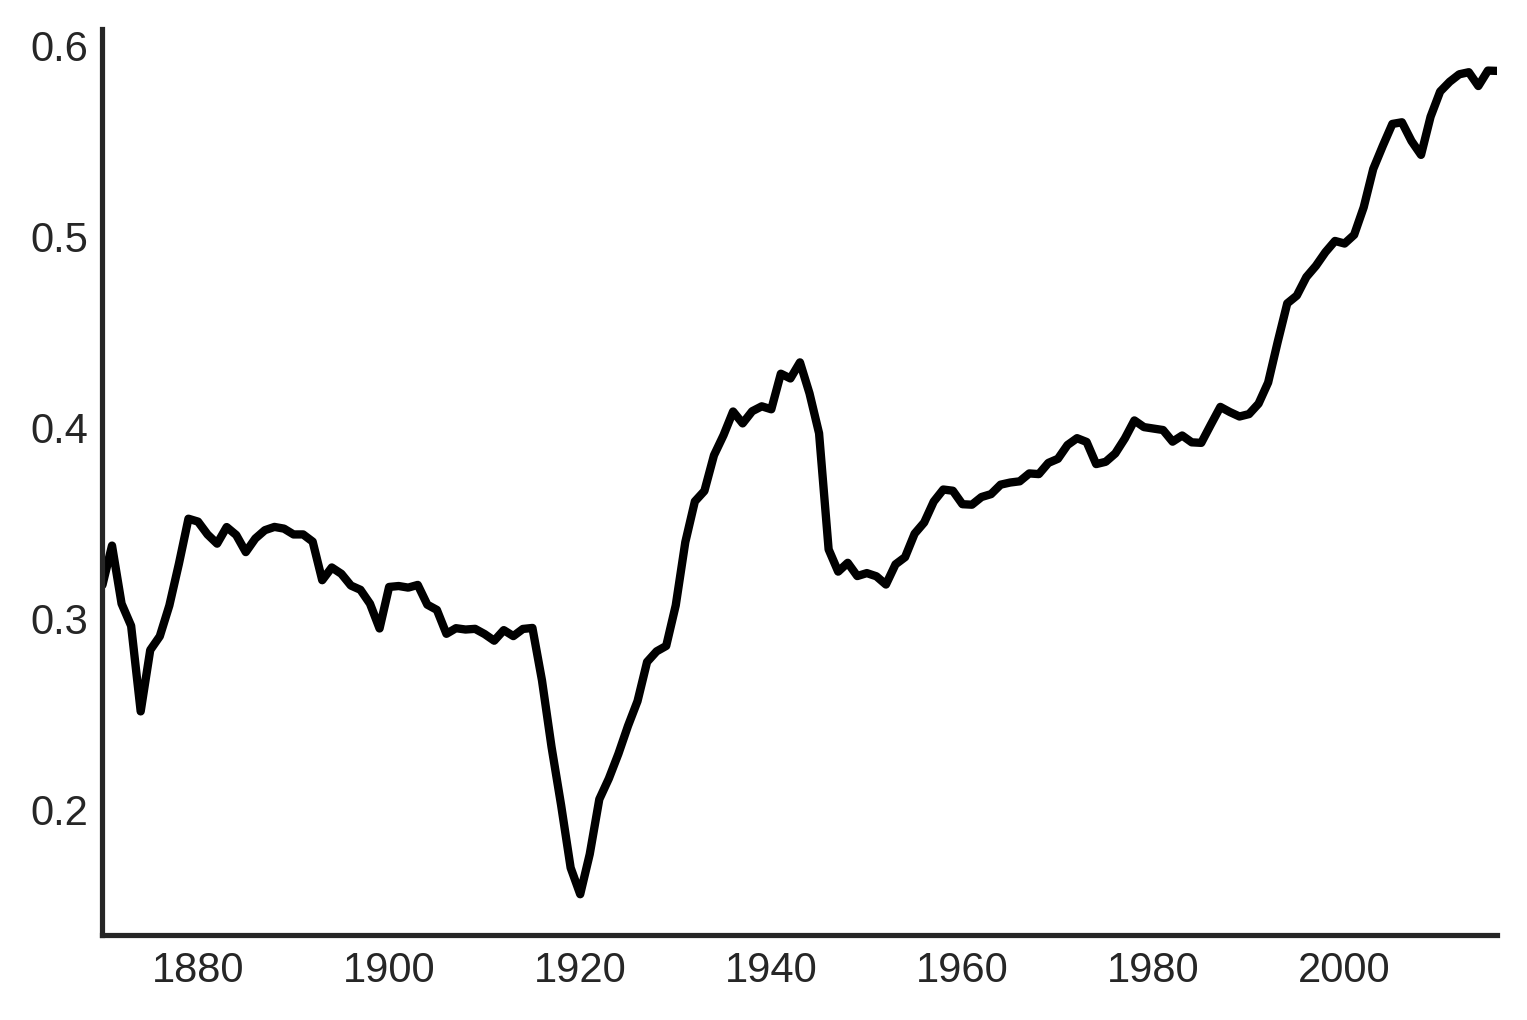
\includegraphics[width=.7\textwidth]{Jorda_Mean.png}
	\caption*{\textbf{Fonte:} \textcite[p.~10]{jorda_great_2014}}
\end{figure}


Recentemente, parte da literatura econométrica também tem lançado luz sobre a importância do investimento residencial para o ciclo econômico\footnote{Além da importância do investimento residencial para a dinâmica econômica, cabe pontuar a relevância da taxa de aquisição de imóveis na determinação do endividamento das famílias e, portanto, destacar a importância de se estudar o tema \cite{schwartz_politics_2009}.
}. \textcite{alvarez_does_2010}, por exemplo, concluem que tal tipo de investimento antecede o ciclo econômico para o caso espanhol e resultados semelhantes podem ser encontrados para França, Espanha  e Itália enquanto o caso alemão apresenta uma dinâmica distinta \cites{ferrara_cyclical_2010}{ferrara_common_2010}. 
Outros estudos empíricos, por sua vez, têm enfatizado o efeito riqueza --- via valorização dos imóveis --- sobre o consumo e indicam tais canais de transmissão são mais incidentes, em ordem, sobre Estados Unidos e Grã Bretanha e mais brandos no caso francês e alemão \cites{sastre_assessment_2010}{chauvin_wealth_2010}{bassanetti_effects_2010}{arrondel_housing_2010}.

A pluralidade de resultados reportada acima sugere que a especificidade institucional de cada país desempenha um papel central nas implicações macroeconômicas do investimento residencial e, portanto, carece de uma análise mais detalhada. A título de exemplo, \textcite{wijburg_alternative_2017} destacam que o mercado imobiliário alemão\footnote{
	\textcite{wijburg_alternative_2017} também apontam que os preços dos imóveis na Alemanha estagnaram enquanto o resto do mundo presenciou um aumento. No entanto, observa-se um movimento recente de aumento nos preços no país, indicando uma maior relevância do tema em um futuro próximo.} é um contra ponto ao ameriacano\footnote{
	A metodologia utilizada por \textcite{wijburg_alternative_2017} é a das ondas de financeirização em que a última onda iniciou no fim da CFG. Dito isso, os autores negam a ideia de que o mercado imobiliário alemão não é financeirizado uma vez que a financeirização imobiliária pode assumir várias formas.}:

\begin{quote}
	\textit{On the one hand, the German housing market was one of the few markets in Western Europe that was not severely affected by the global housing boom of the early 2000s. On the other hand, recent developments suggest that the role of finance in the German housing system is \textbf{changing}, but not in the same way as in other countries} \cite[p.~969, grifos adicionados]{wijburg_alternative_2017}
\end{quote} 


Sendo assim, cabe destacar a importância das instituições\footnote{
	Ao longo desta pesquisa, adota-se a definição de instituições como em 	\textcite[p.~85]{dequech_economic_2013}: ``\textit{Institutions are broadly understood here as socially shared systems of rules of behavior or of thought that have some recurrence}'' e, mais especificamente, serão avaliadas as instituições formais.} 
para a compreensão das inter-relações entre o mercado imobiliário e o de crédito.  
%No que diz respeito ao arranjo institucional do mercado imobiliário, seja ele micro ou macro econômico, influencia principalmente nas formas que os credores (bancos e investidores institucionais) administram o risco e os custos dos empréstimos hipotecários. 
Seguindo este tipo de análise, \textcite{van_gunten_varieties_2018} argumentam que as mudanças institucionais foram responsáveis pela maior intensificação financeira --- maior endividamento das famílias e não um aumento no número de famílias endividadas --- em Portugal e Espanha se comparado com França e Alemanha\footnote{\textcite[p.~92]{van_gunten_varieties_2018} também pontuam a especificidade do caso alemão em que houve um ``desintensificação financeira''.}. Dentre os principais determinantes institucionais a serem analisados, destaca-se: (i) possibilidade de transferência de riscos (\textit{e.g.} securitização\footnote{Para uma descrição do aumento da securitização nos Estados Unidos, ver \textcite{green_american_2005} e \textcite{cagnin_o_2009}.}) que têm aumentado entre os países europeus \cite{european_central_bank_housing_2010}; (ii) disponibilidade de crédito de longo-prazo para as famílias \cite{schwartz_politics_2009}; (iii) duração das hipotecas e existência de um mercado secundário \cite{green_american_2005}; (iv) determinação  e tipo da taxa de juros das hipotecas (fixa ou flexível); (v) arranjo regulatório sobre reembolso antecipado (contrato ou legislação) e formas de refinanciamento e; (vi) acesso a linhas de crédito, ou seja, permissividade da retirada do capital próprio (\textit{equity withdrawal contracts}). Dentre os itens elencados anteriormente (organizados na tabela \ref{Institucional} para alguns países), destaca-se o acesso a linhas de crédito através das hipotecas cuja relevância é maior para o caso norte-americano --- pelos efeitos significativos já mencionados sobre o ciclo econômico --- e por serem mais incomuns nos países europeus \cite[p.~95]{van_gunten_varieties_2018}.

\begin{table}[htb]
	\centering
	\caption{Características institucionais de alguns países europeus}
	\label{Institucional}
	\resizebox{\textwidth}{!}{%
		\begin{tabular}{l|c|c|c|c|c|c}
			\hline \hline\\
			\textbf{Fatores institucionias}                                                              & \multicolumn{1}{c}{\textbf{França}} & \multicolumn{1}{c}{\textbf{Alemanha}} & \multicolumn{1}{c}{\textbf{Itália}} & \multicolumn{1}{c}{\textbf{Holanda}} & \multicolumn{1}{c}{\textbf{Portugal}} & \multicolumn{1}{c}{\textbf{Espanha}} \\\hline
			Maturidade das hipotecas                                                                       & 19                                  & 25-30                                 & 22                                  & 30                                   & 30-40                                 & 30                                   \\\hline
			Tipo de taxa de juros                                                                        & Fixa                                & Fixa                                  & Variável                            & Fixa                                 & Variável                              & Variável                             \\\hline
			\begin{tabular}[c]{@{}l@{}}Reembolso antecipado:\\ Contrato (C)/ Legislação (L)\end{tabular} & C/L                                 & C/L                                   & L                                   & C                                    & L                                     & C/L                                  \\\hline
			\begin{tabular}[c]{@{}l@{}}Retirada de capital próprio \\ (Permissão)\end{tabular}           & Não                                 & Não                                   & Não                                 & Sim                                  & -                                     & Limitado                             \\\hline
			\begin{tabular}[c]{@{}l@{}}Financiamento pelo \\ mercado de capitais\end{tabular}            & 12\%                                & 14\%                                  & 20\%                                & 25\%                                 & 27\%                                  & 45\%                                 \\\hline
			\begin{tabular}[c]{@{}l@{}}Execução hipotecária (\textit{Foreclosure}): \\ duração (meses)\end{tabular}             & 20                                  & 9                                     & 56                                  & 5                                    & 24                                    & 8 \\ \hline\hline                                 
		\end{tabular}%
	}
\caption*{\textbf{Fonte:}  \textcite[p.~94, adaptado e traduzido]{van_gunten_varieties_2018}}
\end{table}



Pontuada a importância do investimento residencial e a relevância das instituições para compreendê-lo, cabe inspecionar a forma com que a heterodoxia tratou do tema. Parte significativa desta literatura  --- emergente no pós-crise imobiliária --- centra esforços na conexão deste tipo de gasto com processos mais gerais como a financeirização \cites{aalbers_financialization_2008}{bibow_financialization_2010} enquanto uma fração minoritária o relaciona com as variabilidades de capitalismo e as relações com o \textit{welfare state} \cite{schwartz_politics_2009}. 
No entanto, a partir da revisão bibliográfica, verificou-se que uma fração pequena da literatura heterodoxa\footnote{
	A título de menção, vale destacar também o trabalho de \textcite{zezza_u.s._2008} em que são investigados os efeitos distributivos sobre o crescimento para a economia norte-americana a partir da metodologia \textit{Stock-Flow Consistent}.}
aborda as relações entre crescimento e investimento residencial que, e isto é central para a análise, não cria capacidade produtiva ao setor privado\footnote{A título de nota, destaca-se que debate ortodoxo sobre desenvolvimento e investimento residencial centrado na década de 60-70 (ver \textcite{arku_housing_2006}) se restringiu em categorizá-lo como um gasto absorvedor de recursos produtivos e indicava  a possibilidade de um sobreinvestimento residencial \cites{solow_importance_1995}{mills_has_1987}. }. 
Uma forma de incluir esse gasto nos modelos de crescimento heterodoxos é a de \textcite{da_silveira_investimento_2019} em que os autores utilizam o supermultiplicador sraffiano (SSM em inglês) por estabelecer um papel fundamental aos gastos autônomos que não criam capacidade no crescimento econômico e na acumulação de capital\footnote{Na contribuição original de \textcite{serrano_sraffian_1995} e nas apresentações mais recentes \cite{freitas_growth_2015}, o modelo é apresentado de modo bastante parcimonioso para evidenciá-lo como um fechamento alternativo, dentro da tradição da teoria do crescimento liderada pela demanda \cite{serrano_sraffian_2017}.}. 
%Nesta família de modelos: 
%	(i) o grau de utilização converge ao normal no longo prazo; 
%	(ii) a distribuição renda tem efeitos de nível apenas e; 
%	(iii) a taxa de crescimento da economia converge a taxa de crescimento dos gastos autônomos. 


A partir do estabelecimento do SSM, algumas questões são colocadas: quais são esses gastos autônomos e quais seus determinantes? Qual o padrão de financiamento e suas consequências? \textcite{pariboni_household_2016} e \textcite{fagundes_dinamica_2017}, por exemplo, avançaram em detalhar o consumo financiado por crédito.  \textcite{brochier_supermultiplier_2018}, por sua vez, incorporam o SSM em uma estrutura contábil mais completa, o arcabouço de consistência entre fluxos e estoques (SFC, na sigla em inglês), para compreender a dinâmica do consumo a partir da riqueza. Por mais que a contribuição de \textcite{da_silveira_investimento_2019} lance luz sobre a inclusão do investimento residencial nesta família de modelos, carece de uma relação entre o mercado imobiliário e de crédito bem como uma maior ênfase no endividamento das famílias e, portanto, tal contribuição precisa ser melhor explorada e estendida.

Como será discutido adiante, a ênfase em tratar a abordagem SFC enquanto uma metodologia decorre da flexibilidade de incluir inúmeras teorias e propostas apesar da rigidez de seus procedimentos. Apenas para elencar alguns temas caros a heterodoxia, tal abordagem trata, mesmo que em sua forma mais originária\footnote{A forma originária dessa família de modelos é encontrada em \textcite{godley_macroeconomics_1983}.}, as formas de financiamento das firmas \cites{asimakopulos_kalecki_1983}{skott_finance_1988}{messori_financing_1991}; endogeneidade da moeda e importância do sistema bancário \cites{messori_financing_1991}{dow_horizontalism:_1996}{arestis_theoretical_1996}{godley_money_1999}; endividamento, distribuição de renda e, apenas para restringir os temas, financeirização \cites{palley_inside_1996}{wolfson_irving_1996}{palley_money_1997}{palley_financial_2002}{dos_santos_revisiting_2009}{palley_inside_2010}{hein_finance-dominated_2012}.

A mesma variabilidade de temas passíveis de serem abordados pela metodologia SFC se estende para a pluralidade dos ativos e do grau de complexidade financeira de cada modelo. Uma forma de visualizar tal flexibilidade é por meio da figura \ref{Heatmap} em que são mapeados os ativos mais frequentes. No entanto, este gráfico também revela que a literatura não dá a devida atenção ao investimento residencial\footnote{Deve ser pontuada a notória exceção de \textcite{zezza_u.s._2008} em que é apresentado um modelo com imóveis em um aparato Kaleckiano enfatizando as implicações distributivas mas não trata de questões envolvendo ganhos de capital ou dos determinantes do investimento residencial.}, sendo o ativo menos estudado. Portanto, fica evidenciada a lacuna que esta pesquisa procurará preencher.

\begin{figure}
	\centering
	\caption{Mapa de calor dos ativos modelados com SFC}
	\label{Heatmap}
	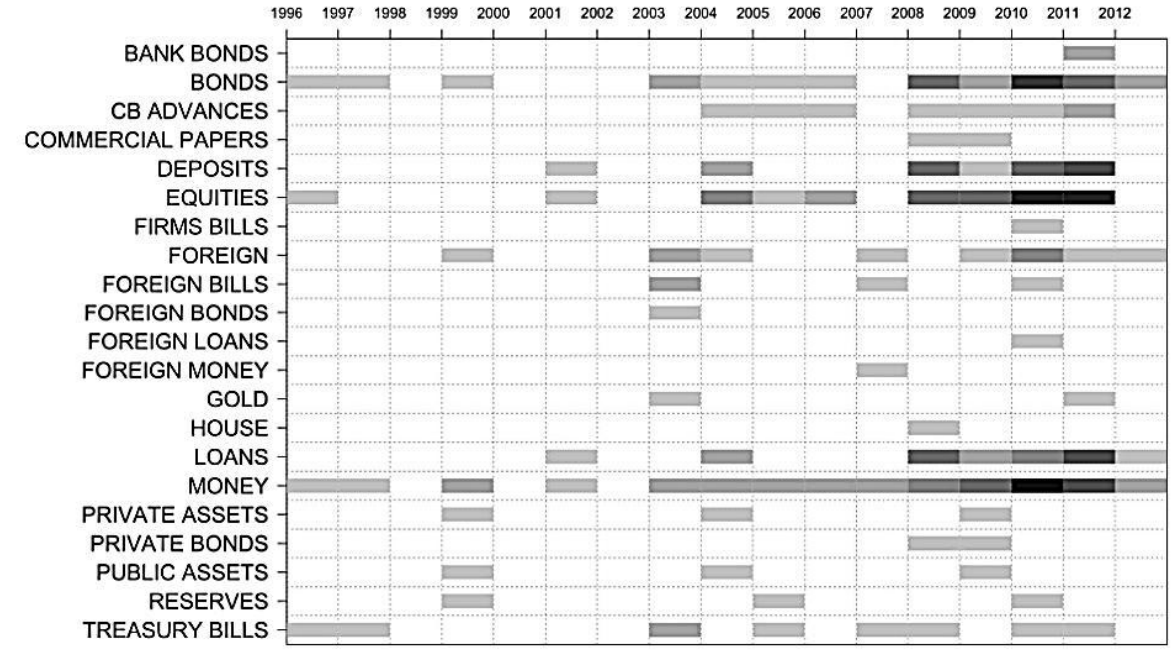
\includegraphics[width = 0.9\textwidth]{../../Escrita_Dissertacao/Da_Silveira_Dissertacao_Atual/Modelo/Caverzassi_Heatmap.png}
	\caption*{\textbf{Fonte:} \textcite[p.~4]{caverzasi_stock-flow_2013}}
\end{figure}


Uma forma de conectar o investimento residencial com o modelo do supermultiplicador sraffiano é por meio da taxa própria de juros dos imóveis (Taxa Própria) desenvolvida por \textcite{teixeira_crescimento_2015} para avaliar o caso norte americano e é definida como a taxa de juros hipotecária ($r_{mo}$) deflacionada pela inflação dos imóveis ({$\dot p_h$}) de modo que o investimento residencial, autônomo e não criador de capacidade produtiva, cresce a taxa $g_Z$ dada por:
\begin{equation}
g_Z = \phi_0 - \phi_1 \overbrace{\left(\frac{1+r_{mo}}{1+\dot p_h} - 1\right)}^{\text{Taxa Própria}}
\end{equation}
em que os $\phi_i$s são parâmetros e cujo termo em parênteses é a Taxa Própria. O primeiro parâmetro se refere aos determinantes de longo prazo (\textit{e.g.} arranjos institucionais do mercado imobiliários e de crédito) enquanto o segundo capta a demanda por imóveis decorrente das expectativas de ganhos de capital resultantes da especulação com o estoque de imóveis existente e diz respeito ao ciclo econômico.

Em outras palavras, a taxa de juros das hipotecas capta o serviço da dívida para os ``investidores'' (neste caso, famílias) enquanto a variação do preço dos imóveis permite incorporar mudança no patrimonio líquido. Portanto, aufere de modo satisfatório o custo real em imóveis de se comprar imóveis \cite[p.~53]{teixeira_crescimento_2015}. Desse modo, a partir da taxa própria de juros do imóveis é possível revelar importância do investimento residencial para além do ciclo e estendê-la para o longo prazo.  Tal proposta, portanto, lança luz sobre a influência da inflação imobiliária na construção de novos imóveis e, de acordo com o supermultiplicador sraffiano, sobre o produto como um todo. 

Como mencionado anteriormente, a referida taxa própria dos imóveis foi desenvolvida para examinar a bolha de ativos ocorria nos EUA e, portanto, não foi feita uma investigação a despeito da aplicabilidade para outros países e este é um dos objetivos desta pesquisa. Além disso, uma vez que a dívida hipotecária é o principal componente do endividamento das famílias, se faz necessária uma melhor compreensão da conexão entre o investimento residencial com as formas de financiamento e estoques financeiros de forma integrada. Nesses termos, a abordagem SFC se mostra a mais adequada para este tipo de análise. Sendo assim, um modelo de crescimento do tipo SSM com a metologia SFC (adiante, SSM-SFC) se mostra com uma alternativa para tratar do investimento residencial em que são mapeadas as relações financeiras entre os diferentes agentes institucionais.


%PERGUNTA
Compreendido este panorama, a presente investigação pretende responder a seguinte pergunta: quais os principais determinantes institucionais que explicam as especificidades do caso norte-americano frente aos demais países da OCDE a despeito das implicações macroeconômicas do investimento residencial? Como conectar o mercado imobiliário e de crédito em um modelo SSM-SFC? 
Portanto, esta pesquisa segue o caminho aberto por \textcite{brochier_supermultiplier_2018} ao adicionar um tratamento adequado das relações financeiras no SSM por meio da metodologia SFC estentendo as contribuições de: 
(i) \textcite{jorda_great_2014} ao investigar o processo de ``hipotecarização'' sob um prisma pós-keynesiano; 
(ii) \textcite{serrano_sraffian_1995} ao incluir o investimento residencial na agenda de pesquisa do supermultiplicador sraffiano; 
(iii) \textcite{teixeira_crescimento_2015} ao avaliar a aplicabilidade da taxa própria de juros para além dos Estados Unidos e;
(iv) \textcite{da_silveira_investimento_2019} ao conectar as relações entre o mercado imobiliário e de crédito diante das especificidades institucionais destacas anteriormente. 
%\section{Objetivos}\label{OBJ}

\begin{description}
	\item[Objetivo geral] Investigar os arranjos institucionais do mercado imobiliário e de crédito dos países da OCDE e investigar as implicações sobre o investimento residencial e contrastá-las com o caso norte-americano
	\item[Objetivos específicos] {\color{white} Texto em branco para espaçamento}
	\begin{itemize}
		\item Examinar o processo de ``hipotecarização'' destacado por \textcite{jorda_great_2014};
		\item Comparar o caso norte-americano com os demais países da OCDE;
		\item Testar a aplicabilidade da taxa própria de juros dos imóveis desenvolvida por \textcite{teixeira_crescimento_2015} para os países da OCDE; 
		\item Detectar os principais determinantes macroeconômicos do investimento residencial por meio de um modelo de dados em painel com auxílio da base de dados desenvolvida por \textcite{jorda_great_2014};
		\item Construir um modelo SFC com supermultiplicador sraffiano cujo gasto autônomo é o investimento residencial e replicar as referidas características institucionais do mercados de crédito e imobiliário.
	\end{itemize}
\end{description}


Para atender estes objetivos, a pesquisa proposta será dividida em três frentes cada qual com seu respectivo capítulo.
A primeira delas trata da inserção e contextualização do investimento residencial em processos mais estruturais como a financeirização em contraposição a ``hipotecarização''. Para isso, serão analisadas as especificidades dos países em questão no que diz respeito ao mercado imobiliário e sua conexão com o mercado de crédito bem como a regulação de preços dos imóveis. Em outras palavras, caberá a este capítulo investigar o quão destoante é o caso norte-americano frente aos demais, com especial ênfase ao caso alemão. Compreendidas as especificidades institucionais de cada país, o capítulo seguinte irá analisar os determinantes do investimento residencial por meio de um modelo de dados em panel. Com isso, esses dois capítulos fornecem o embasamento qualitativo e quantitativo para o modelo teórico que será desenvolvido no terceiro capítulo da tese. A partir da metodologia \textit{Stock-Flow Consistent} (SFC), serão testados os diferentes arranjos institucionais destacados no capítulo primeiro bem como os determinantes do investimento residencial reportados no capítulo segundo e, assim, conectar com a literatura do supermultiplicador sraffiano. Sendo assim, cabe a seção seguinte esclarecer as etapas da metodologia SFC.

\section{Objetivos}\label{OBJ}

\begin{description}
	\item[Objetivo geral] Analisar a dinâmica da economia brasileira em termos de crescimento nos anos de 2000-2014 com ênfase nas mudanças redistributivas observadas assim como identificar os fatores que explicam esta trajetória; {\color{blue} Muito geral?}
	\item[Objetivos específicos:] (i) Investigar as diferentes teorias de crescimento heterodoxas e suas respectivas relações com distribuição de renda; (ii) Apresentar a teoria monetária da distribuição de \textcite{pivetti_essay_1992} assim como suas limitações e adequar este arcabouço teórico ao Brasil; (iii) Explorar as mudanças na distribuição pessoal e funcional da renda no caso brasileiro; (iv) Dialogar com a literatura assim como expor suas respectivas limitações e  diferenças argumentativas em relação ao objetivo geral apresentado; (v) Explicitar os impactos da ampliação do crédito ao consumidor, valorização do salário mínimo e determinação da taxa de juros à luz da teoria monetária da distribuição e; (vi) Examinar a economia brasileira com base no modelo do supermultiplicador sraffiano a partir de simulações computacionais. {\color{blue} Especificar mais?}
\end{description}




%\section{Metodologia, materiais e análise}\label{Metodo}

A pesquisa proposta será dividida em três frentes cada qual com seu respectivo capítulo.
A primeira delas trata da relação entre distribuição de renda e crescimento. A segunda, por sua vez, irá abordar os nexos entre distribuição pessoal e funcional da renda e crédito tendo em vista as mudanças distributivas verificadas na economia brasileira. Por fim, serão estudadas as relações entre crédito e crescimento. 
Dessa forma, a dissertação será composta por três capítulos além da introdução e das conclusões.  


Compreendidos os objetos e objetivos de cada um dos capítulos, são explicitadas as formas em que serão realizados. O capítulo primeiro tem aspectos teóricos que servirão de base para a análise desempenhada no capítulo seguinte.
Dessa forma, esses conceitos são fundamentais por descrever e situar o tema desta pesquisa em um campo mais geral em que serão evidenciadas as discussões da literatura especializada assim como suas limitações. 

Sendo assim, este capítulo irá rever as teorias heterodoxas de crescimento dando ênfase aos elementos referentes à distribuição de renda. Para isso, serão apresentados os seguintes modelos: (i) Neo-Keynesiano; (ii) Pós-Keynesiano; (iii) supermultiplicador sraffiano\footnote{Partindo de \textcite[Capítulo 6]{lavoie_post-keynesian_2014}, considera-se os termos neo-Keynesianos e modelo de Cambridge como sinônimos assim como Pós-Keynesianos e modelo Neo-Kaleckiano. Além disso, dados os objetivos desta pesquisa, o SSM será apresentado em maior detalhe.}. Dito isso, segue uma breve apresentação destes modelos.

%=================================================================================
%								Cambridge
%=================================================================================

A família de modelos Neo-Keynesianos desenvolvida por Kaldor, Robinson e Passinetti surge de uma tentativa de estender o princípio da demanda efetiva (PDE) para o longo prazo assim como para ser uma alternativa às teorias marginalistas. No entanto, esses modelos supõem que a economia opera à plena utilização da capacidade no longo prazo e, como consequência, o sistema econômico está na fronteira salário-lucro. Além disso, nesses modelos o investimento é tratado exogenamente e, como resultado, é a taxa de lucros ($r$) que determina a taxa de acumulação ($g$) \cite[Capítulo 6]{lavoie_post-keynesian_2014}. Em outras palavras, o padrão de crescimento é \textit{profit-led} em que restrições do lado da oferta persistem inclusive no longo prazo.

Dito isso, a Eq \ref{Cambridge} apresenta este modelo em que a taxa de crescimento da poupança ($g^s$) é determinada pela propensão a poupar sobre os lucros ($s_p$) e pela taxa de lucro ($r$). A taxa de crescimento do investimento, por sua vez, depende tanto de parâmetros comportamentais que expressam os \textit{animal spirits} ($\gamma$) quanto da sensibilidade  da taxa de crescimento em relação aos lucros esperados ($\gamma_rr^e$).

\begin{equation}
\label{Cambridge}
\begin{cases}
g^s = s_pr\\
g^i = \gamma + \gamma_rr^e
\end{cases} \Rightarrow g^* = \frac{s_p\gamma}{(s_p-\gamma_r)} \Rightarrow r^* = \frac{\gamma}{(s_p - \gamma_r)}
\end{equation}

Em equilíbrio de longo prazo (\textit{i.e.} $r = r^e$), existe uma taxa de crescimento de equilíbrio ($g^*$) compatível com uma taxa de lucro desejada ($r^*$). A estabilidade deste modelo, por sua vez, depende que a função investimento seja menos inclinada que a função poupanças, ou seja, $\gamma_r < s_p$. Resta, no entanto, explicitar como essa família de modelos se relaciona com distribuição de renda.

Analisando as contribuições de Kaldor, \textcite{hein_distribution_2014} destaca que a propensão a poupar que determina a taxa de lucro é resultada de uma média ponderada das propensões dos capitalistas e trabalhadores. Sendo assim, mudanças na distribuição funcional da renda alteram a taxa de lucro que, por sua vez, influencia a taxa de crescimento. Nesses termos, há uma simultaneidade entre distribuição e acumulação, ou seja, a distribuição de renda é endógena. Não apenas isso, mas dada a hipótese de que a economia opera ao pleno-emprego, há uma relação negativa entre \textit{wage-share} e \textit{profit-share}. Considerando que a rigidez dos salários é maior que a dos preços, a taxa de lucro torna-se residual. Portanto, o fechamento econômico deste modelo decorre da distribuição de renda que ajusta a poupança ao investimento. 

%=================================================================================
%								Neo-Kaleckiano: 2 parágrafos
%=================================================================================

Isto posto, cabe destacar que os modelos neo-Keynesianos foram alvo de diversas críticas que, em grande medida, realçam as inconsistências lógicas entre o PDE e as conclusões do modelo. Os autores Neo-Kaleckianos, por sua vez, dirigiram suas críticas à ausência de uma estrutura de mercado oligopolizada e à convergência do grau de utilização da capacidade ao nível de pleno-emprego. Em resposta, surgem os modelos Pós-Keynesianos em que o grau de utilização da capacidade é endogeneizado e a determinação das parcelas da renda dependem do \textit{mark-up}.

Apesar das diferentes versões desta famílias de modelos, \textcite[p.~360]{lavoie_post-keynesian_2014} afirma que existem quatro elementos comuns: (i) investimento depende do nível de utilização da capacidade ($u$); (ii) preços são determinados via \textit{cost-plus pricing} e não como decorrência das forças de mercado; (iii) propensão marginal a poupar dos trabalhadores é menor do que dos capitalistas e normalmente nula e; (iv) não há convergência à plena-capacidade e oferta de trabalho não é uma restrição.

Dito isso, é possível apresentar o modelo neo-kaleckiano básico em que a taxa de lucro ($r$) é determinada pelo grau de utilização ($u$), pelo \textit{profit-share} e pelo inverso da relação capital-produto ($v$). A taxa de crescimento da poupança ($g^s$) é definida tal como no modelo de Cambridge. Por fim, a taxa de crescimento do investimento depende tanto de parâmetros comportamentais (\textit{e.g. animal spirits}, $\gamma$) quanto da sensibilidade do investimento em relação aos desvios do grau de utilização do nível esperado ($\gamma_u(u^e-u_n)$):
 
\begin{equation}
\begin{array}{ll}
r = \pi u / v\\
g^s = s_p\pi u/v\\
g^i = \gamma + \gamma_u(u^e-u_i)
\end{array}
\end{equation}

Neste modelo, o equilíbrio de longo prazo é atingido quando a taxa de crescimento da poupança ($g^s$) se iguala à do investimento ($g^i$), mas para isso depende que a poupança seja mais sensível do que as mudanças no grau de utilização da capacidade ($s_p\pi > v\gamma_u$). Neste ponto, a taxa de utilização esperada ($u^e$) é igual à corrente ($u_i$), ou seja, o equilíbrio ocorre quando as expectativas em relação ao grau de utilização são realizadas. Portanto, a poupança se ajusta ao investimento quando $u_i = u^e$, ou seja, o grau de utilização da capacidade é o fechamento deste modelo.

No entanto, dados os objetivos desta pesquisa, cabe pontuar quais são os determinantes da distribuição de renda nestes modelos. Como destaca \textcite[Capítulo 5]{hein_distribution_2014}, a parcela nos lucros na renda ($\pi$) é determinado pelo \textit{mark-up} ($\theta$) que, por sua vez, depende da estrutura de mercado. Sendo assim, a distribuição da renda é macroeconomicamente exógena, mas microfundamentada.

Isto posto e considerando a grande aderência deste modelo na tradição heterodoxa,  é esperado que seja alvo de críticas e adaptações. Dentre elas, cabe ressaltar a de \textcite{bhaduri_unemployment_1990} em que os autores colocaram em questão a não capacidade desses modelos em explicar o porquê do aumento do grau de utilização da capacidade mesmo quando o \textit{profit-share} é constante. Dito isso, os autores modificam a função investimento do modelo Kaleckiano canônico e concluem que o regime de acumulação pode ser tanto \textit{wage} quanto \textit{profit-led}, mas em ambos o investimento é a variável que determina crescimento econômico. 


%=================================================================================
%								SSM
%=================================================================================
Outro conjunto de críticas, por sua vez, decorre da hipótese de endogeinização do grau de utilização da capacidade. Seguindo as contribuições de Garegnani, alguns autores sraffianos questionam o porquê desta variável não convergir ao normal no longo prazo. Grosso modo, essa linha argumentativa defende que tanto a subutilização quanto a sobreutilização da capacidade são prejudiciais dada a concorrência capitalista. Em resposta tanto ao modelo de Cambridge quanto a família de modelos neo-kaleckianos, \textcite{serrano_sraffian_1995} elabora o modelo do supermultiplicador sraffiano  (adiante, SSM).

Em linhas gerais, o SSM descreve um padrão de crescimento liderado pela demanda em que os gastos não criadores de capacidade produtiva (ditos improdutivos) determinam a taxa de crescimento de longo prazo. Além disso, neste modelo, o grau de utilização da capacidade produtiva ($u_t$) tende, via concorrência, ao normal ($\mu$) no longo prazo\footnote{\textcite{nikiforos_comments_2018} argumenta que a convergência do grau de utilização da capacidade ao nível desejado tem contribuições para as teorias heterodoxas de crescimento que podem ser verificadas pelos esforços de autores neo-kaleckianos em incluí-la sem perder a essência do modelo, ou seja, ajuste endógeno de $u$.}.
Dito isso, seja $Z_t$ o componente autônomo da demanda agregada financiado por crédito em $t$; $h_t$ a propensão marginal a investir e; $s$ a propensão marginal à poupar:

\begin{equation}
Y_t = \left( \frac{1}{s-h_t} \right)\cdot Z_t
\label{SSM}
\end{equation}
A equação \ref{SSM} indica que os efeitos dos gastos improdutivos sobre o produto agregado ($Y_t$) são capturados pelo termo em parênteses denominado de supermultiplicador sraffiano. Seguindo a exposição de \textcite{serrano_sraffian_2017}, a Eq \ref{SSM_g} mostra a dinâmica da taxa de crescimento da economia ($g_t$) para uma dada taxa dos componentes autônomos da demanda mencionados ($g_z$) em que o ajuste do estoque de capital fixo em relação à capacidade produtiva é feito de forma tênue pelo parâmetro $\gamma$

\begin{equation}
g_t = g_z + \frac{h_t\gamma(u_t-\mu)}{s-h_t}
\label{SSM_g}
\end{equation}
No longo prazo, portanto, com a taxa de utilização da capacidade tendendo ao nível desejado (\textit{i.e.} $u_t = \mu$) implica que é a taxa de crescimento da economia é dada por $g_z$.

No entanto, resta especificar como este mecanismo ocorre. \textcite{serrano_sraffian_1995} demonstra que a possibilidade de ajuste endógeno da razão entre a propensão média ($S{Me}$)  e marginal à poupar ($s$). Essa endogeneidade, por sua vez, advém da existência de gastos autônomos que não criam capacidade \cite{serrano_sraffian_2017}. 
Em outras palavras, para uma dada propensão marginal à poupar ($s$), a poupança média se ajusta ao investimento que, por sua vez, é induzido pela necessidade de adaptar o grau de utilização da capacidade ao nível normal por conta da concorrência capitalista.  A forma com que este investimento induzido garante o nível adequado da propensão média à poupar se dá por meio do supermultiplicador. 

Dessa forma, tal como aventado pelo princípio da demanda efetiva, o supermultiplicador sraffiano possibilita que a propensão marginal à investir determine a poupança.
Com isso, restaura-se um regime de acumulação liderado pela demanda em que a distribuição de renda é determinada pela teoria sraffiana e o nível de utilização da capacidade tende ao normal \cite{nikiforos_comments_2018}. 

%=================================================================================
%								Tabela: modelos de crescimento
%=================================================================================
\begin{table}[htb]
	\centering
	\caption{Teorias do crescimento e distribuição de renda}
	\label{crescimento}
	\resizebox{\textwidth}{!}{%
		\begin{tabular}{l|c|c|c|c|c|l}
			\hline \hline
			Modelo & \begin{tabular}[c]{@{}c@{}} Padrão de \\crescimento \end{tabular} & \begin{tabular}[c]{@{}c@{}} Condição de\\ estabilidade \end{tabular} & \begin{tabular}[c]{@{}c@{}} Distribuição \\de renda \end{tabular} & \begin{tabular}[c]{@{}c@{}}Grau de utilização \\ da capacidade\end{tabular} & \begin{tabular}[c]{@{}c@{}} Capacidade  \\ produtiva \end{tabular} & \begin{tabular}[l]{@{}l@{}} Hipótese Keynesiana \\ (Ajuste S-I) \end{tabular} \\ \hline
			Cambridge & \begin{tabular}[c]{@{}c@{}} \textit{Profit-led} \\ (Restrições de oferta) \end{tabular} & $\gamma_r < s_p$ & Endógena & \begin{tabular}[c]{@{}c@{}} Exógena \\(pleno-emprego) \end{tabular} & Exógena& \begin{tabular}[l]{@{}l@{}}Via distribuição \\funcional da renda\end{tabular}\\  \hline
			Neo-Kaleckiano & \begin{tabular}[c]{@{}c@{}} Wage/Profit-led \\(via investimento)\end{tabular} & $s_p\pi>v\gamma_u$ & \begin{tabular}[c]{@{}c@{}} Exógena \\ (\textit{Mark-up}) \end{tabular} & Endógena   & Exógena &  \\ \hline
			\begin{tabular}[l]{@{}l@{}}Supermultiplicador \\Sraffiano \end{tabular} & \begin{tabular}[c]{@{}c@{}} Demand-led \\(via consumo)\end{tabular} & $\Downarrow \gamma$& \begin{tabular}[c]{@{}c@{}} Exógena \\ (Teoria Sraffiana)  \end{tabular} & \begin{tabular}[c]{@{}c@{}} Exógena \\(Tende ao normal) \end{tabular}  & Endógena & \begin{tabular}[c]{@{}l@{}} Via \textit{fraction} ($f$)\\ $f = s/S_{Me}$ \end{tabular} \\ \hline \hline
		\end{tabular}%
	}
\caption*{\textbf{Fonte:} Elaboração própria}
\end{table}


%=================================================================================
%								Pivetti
%=================================================================================
Dito isso, a Tabela \ref{crescimento} resume os modelos de crescimento anteriormente discutidos. Adiante,
serão avaliadas algumas teorias da distribuição de renda, em especial a teoria monetária da distribuição desenvolvida por \textcite{pivetti_essay_1992}. Partindo das contribuições de \textcite{sraffa_producao_1985}, o autor argumenta que, no longo prazo, é a taxa de juros que regula a taxa de lucro e não o oposto\footnote{Esta constatação é inspirada em autores como Marx e Keynes.}. Dada essa inversão causal, propõe que a taxa de lucro do investimento ($r_a$) é determinada tanto pela taxa de juros,  cuja autoridade monetária tem influência, relevante no longo prazo ($i_{\Delta LP}$) quanto pelo lucro normal do empreendimento ($npe$):

\begin{equation}
r_a = i_{\Delta LP} + npe
\label{pivetti}
\end{equation}

A Eq \ref{pivetti} mostra que taxa de juros e de lucros possuem uma dinâmica semelhante no longo prazo em que a relação causal vai da primeira para a última.
Com isso, dado o grau de liberdade existente na teoria clássica/sraffiana da distribuição de renda, Pivetti propõe que a taxa de juros relevante no longo prazo intermedeia a relação entre preços e salários nominais. 

Grosso modo, nesta abordagem, a
barganha salarial reflete características político-institucionais relevantes para a distribuição de
renda. Tais especificidades impossibilitam a determinação de uma teoria geral para a distribuição. Apesar de relevante, a negociação salarial tem efeitos indiretos sobre a
determinação das parcelas distributivas. Por fim, os efeitos permanentes decorrem de mudanças persistentes na taxa monetária de juros (\textit{i.e.} taxa de juros relevante no longo prazo).
Dessa forma, a política monetária pode ter menor autonomia a depender do poder de
determinadas classes político-econômicas na correlação de forças. 

Portanto, a determinação das parcelas de renda via conflito distributivo é internalizada na especificação da taxa de juros, ou seja, na política monetária. Partindo de um referencial distinto, \textcite{singer_cutucando_2015} avalia como as disputas no governo Dilma foram expressas na redução deliberada da taxa de juros. Sendo assim, fica evidente o potencial explicativo de uma teoria tal como a de \textcite{pivetti_essay_1992} para o caso brasileiro recente. Sendo assim, com esses elementos em mãos, serão destacadas algumas das variáveis macroeconômicas relevantes que, dadas as devidas mediações, auxiliarão a narrativa construída no capítulo seguinte.

No capítulo descritivo, portanto, serão articuladas algumas interpretações das mudanças redistributivas ocorridas no Brasil em que se combinou crescimento, distribuição de renda e inclusão social. Para isso, serão analisadas tanto as políticas econômicas adotadas como seus impactos. Em relação às medidas praticadas, serão examinadas as valorizações reais do salário mínimo, crédito direcionado ao consumo assim como mudanças em algumas taxas de juros selecionadas. Já em relação aos impactos, serão avaliados a participação dos salários na renda, endividamento e consumo das famílias e, especialmente, mudanças distributivas a partir de alguns critérios de riqueza (\textit{i.e.} participação na renda por decis e classe sócio-econômica) assim como dados tributários que forem pertinentes tal como o IRPF. Com isso, objetiva-se destacar os componentes responsáveis pela dinâmica da economia brasileira no período averiguado (2000-14) em termos da distribuição de renda. 

%=================================================================================
%								Brasil
%=================================================================================

%=================================================================================
%								Brasil: Corrêa e dos Santos (2013)
%=================================================================================
{\color{blue} Parágrafo sobre 2000-2004?}


No que refere aos anos de 2004-2010, \textcite{correa_notas_2013} argumentam que houve um processo de crescimento econômico elevado acompanhado tanto de inclusão social quanto de uma maior importância da demanda doméstica. Adiante, alegam que o cenário externo favorável permitiu que tal arranjo fosse possível. No entanto, destacam que a conjuntura internacional foi uma condição necessária mas não suficiente para permitir esta dinâmica. Em especial, as transferências sociais assim como aumento do salário mínimo desempenharam papel fundamental na melhora da distribuição de renda. Em paralelo, como aponta \textcite{dos_santos_notas_2013}, o Estado tomou para si a função de induzir o investimento privado neste período.

%=================================================================================
%								Brasil: Serrano & Summa (2018)
%=================================================================================
Os impactos das mudanças redistributivas elencadas não ficaram restritas à esfera econômica. Avaliando o mesmo período, \textcite{serrano_conflito_2018} pontuam que o arranjo composto de crescimento e inclusão social (denominado pelos autores de ``Breve Era de Ouro'') gerou mudanças significativas no mercado de trabalho\footnote{Em relação o mercado de trabalho, vale destacar o estudo de \textcite{carneiro_politica_2018-1} em que os autores destacam a redução da dispersão salarial não acompanhada de uma mudanças na composição do emprego. Dentre os fatores que melhor explicam essa mudança na distribuição de renda, pontuam elementos institucionais como a formalização do emprego quanto e as políticas salariais adotadas.} ao ponto de causas efeitos indesejados. A redução do desemprego aberto alinhado com aumentos reais do salário mínimo fizeram com que o poder de barganha dos trabalhadores ampliasse. Como consequência, as margens e taxas de lucro reduziram. Desse modo, os efeitos diretos dessa chamada ``revolução indesejada'' são os aumentos consistentes da participação dos salários na renda. Os efeitos indiretos, por sua vez, decorrem da guinada da política econômica iniciada em 2011 de aposta no investimento privado e melhor representada pelo ajuste fiscal de 2015. Argumenta-se que essa alternância de política impactou negativamente a demanda agregada e, consequentemente, provocando a desaceleração (rudimentar) do crescimento \cite{serrano_demanda_2015}.

%=================================================================================
%								Tabela
%=================================================================================

\begin{table}[htb]
\caption{Taxa de juros nominal e real (IPCA), crédito em relação ao PIB e endividamento das famílias em relação à Massa Salarial Ampliada Disponível (2005-2014, média anual em \%)}
	\begin{center}
	\label{tabela_resumo}
	\resizebox{\textwidth}{!}{%
		\begin{tabular}{ccc|ccc|ccc}
			\cline{2-9}
			 &\multicolumn{2}{c}{Selic} &  \multicolumn{3}{c}{Crédito$^a$} & \multicolumn{3}{c}{Endividamento$^b$} \\ \hline \hline
			Ano & Nominal & Real &   Pessoa Física & Pessoa Jurídica & Total & Habitacional & Não habitacional & Total \\
			%2000 &17.59 & 11.62 & - & - & 26.6 & - & - & - \\
			%2001 &17.47 & 9.80 & - & - & 26.67 & - & - & - \\
			%2002 &19.11 & 6.58 & - & - & 25.72 & - & - & - \\
			%2003 &23.37 & 14.07 & - & - & 24.54 & - & - & - \\
			%2004 &16.24 & 8.64 & - & - & 24.75 & - & - & - \\
			2005 & 19.12 & 13.43 & - & - & 26.46 & 3.11 & 17.31 & 20.42 \\
			2006 & 15.28 & 12.14 & - & - & 28.99 & 3.36 & 20.34 & 23.7 \\
			2007 & 11.98 & 7.53 & 14.92 & 17.37 & 31.97 & 3.83 & 23.4 & 27.23 \\
			2008 & 12.36 & 6.46& 16.73 & 20.49 & 37.23 & 4.54 & 27.08 & 31.62 \\
			2009 & 10.06 & 5.75 & 18.00 & 22.84 & 40.84 & 5.68 & 28.29 & 33.97 \\
			2010 & 9.80  & 3.90 & 19.22 & 23.61 & 42.84 & 7.71 & 29.95 & 37.66 \\
			2011 & 11.66 & 5.16 & 20.35 & 24.27 & 44.62 & 9.9 & 31.16 & 41.06 \\
			2012 & 8.53 & 2.70 & 21.65 & 25.63 & 47.28 & 11.93 & 31.13 & 43.06 \\
			2013 & 8.18 & 2.27 & 22.85 & 26.81 & 49.66 & 14.45 & 30.28 & 44.73 \\
			2014 & 10.86 & 4.46& 23.74 & 27.01 & 50.75 & 16.87 & 28.8 & 45.67 \\ \hline \hline
		\end{tabular}%
	}
\end{center}
\footnotesize{$^a$ Por conta de mudanças metodológicas, optou-se por não incluir dados referentes ao crédito à pessoa física e jurídica para os anos de 2005 e 2006.$^b$ Dados referentes ao endividamento das famílias disponíveis a partir de 2005.}\\
\caption*{\textbf{Fonte:} Bacen}
\end{table}


%=================================================================================
%								Brasil: Dos Santos (2013)
%=================================================================================
Em relação à demanda agregada, \textcite{dos_santos_notas_2013} investiga a dinâmica do consumo para os anos 2004-2012. Conclui que há uma relativa estabilidade, mesmo que por construção, do consumo privado em termos do PIB. Além disso, destaca que há uma mudança da importância relativa de bens de consumo duráveis tais como automóveis e eletrodomésticos. A explicação desta dinâmica, argumenta, decorre em grande medida pelo aumento da concessão de crédito e de aproximações da renda disponível assim como pela redução na taxa de juros real. Como consequência, observa-se um aumento do endividamento em relação à Massa Salarial Ampliada Disponível (MSAD).

Os dados apresentados na Tabela \ref{tabela_resumo} ilustram essa trajetória. De um lado, constatam-se diminuições na taxa de juros real (deflacionada pelo IPCA) média de 2005 à 2010 (redução de aproximadamente 50,05\%). De outro, observa-se um aumento tanto no crédito em termos do PIB quanto dos endividamento das famílias em relação à MSAD no mesmo período\footnote{Além disso, vale destacar que enquanto há um aumento simétrico do crédito à pessoa física e jurídica, o endividamento das famílias apresenta um comportamento distinto. Apesar de majoritário, o comprometimento da renda das famílias com serviço da dívida não-habitacional perdeu participação relativa com o crescimento do crédito habitacional decorrentes do Programa Minha Casa Minha Vida. }. 

%=================================================================================
%								Brasil: Fontenele (2016)
%=================================================================================
Vale destacar que outros efeitos da inclusão social podem ser captados pela análise das mudanças no padrão de consumo elencadas anteriormente. \textcite{fontenelle_alcances_2016} parte das jornadas de junho de 2013 para pontuar como movimentos sociais até então focalizados se tornaram uma massa heterogênea que tinham a crítica à oferta pública como ponto em comum. Grosso modo, a autora argumenta que houve uma transformação na reivindicação por cidadania para um embricamento da democracia com o ato de consumir. Em outras palavras, a forma de pensar do consumidor é trasladada ao cidadão \cite{streeck_citizens_2012}. 
A relevância desta discussão para esta pesquisa decorre das transformações do padrão de consumo em que o crédito desempenhou um papel de destaque \cite{schettini_novas_2011}. Em resumo, observa-se tanto uma democratização do consumo quanto um consumo democratizante, ou seja, o consumo mediou a ascensão social. A implicação macroeconômica desta constatação é o já apontado aumento do endividamento das famílias. 



É digno de nota que, tal como \textcite{dos_santos_notas_2013}, argumenta-se que esse maior endividamento não é necessariamente negativo, mas sim, expressa as mudanças redistributivas observadas. Em outras palavras, é esperado que em países neste estágio de desenvolvimento apresentem conjuntamente maior inclusão social seguido de aumento do endividamento.
Tendo em vista esse movimento, foram adotadas em 2010 medidas macroprudenciais para a redução de crédito \cite{ribeiro_o_2016}. O argumento aqui defendido é que essa alternância de política fez com que a demanda agregada e a taxa de crescimento se reduzissem. Como consequência, o endividamento das famílias continuou a aumentar, mas a taxas decrescentes.



%=================================================================================
%								Brasil: Serrano & Summa (2018) 2 - Investimento
%=================================================================================

Além disso, por mais que o consumo doméstico tenha desempenhado um papel importante na dinâmica deste período, o investimento foi o componente que apresentou maiores taxas de crescimento entre 2004-2010 \cite{dos_santos_notas_2013}. Nesse período, portanto, verifica-se a indução do investimento privado decorrente de aumento dos componentes autônomos da demanda tal como o crédito ao consumo.
Como destacam \textcite{serrano_conflito_2018}, a maior participação dos salários na renda e subsequente redução das margens e taxas de lucro não implicaram (nem implicam) em diminuição do investimento. Seguindo o SSM, argumentam que a decisão de investir decorre das perspectivas de demanda futura e não a recomposição das margens de lucro. 


Isto posto, cabe destacar que a
relevância teórica desta constatação é a negação de um \textit{trade-off} entre gasto improdutivo e investimento tão comum na literatura \cite{serrano_acumulacao_2001}. 
Nesses termos, verifica-se que a guinada a favor do investimento privado nos anos 2011-2014 não só foi incapaz de retomar o padrão de crescimento anterior como também fundamentou as bases de sua derrocada \cite{serrano_demanda_2015}. Com isso, revela-se a justificativa e pertinência de se analisar o Brasil à luz do supermultiplicador sraffiano.


%=================================================================================
%								Recorte temporal
%=================================================================================
{\color{blue} Atenção: 2000}

Dito isso, cabe destacar o porquê do recorte temporal adotado, qual seja, 2000-2014. Os anos se referem aos dois mandatos do então presidente Lula e ao primeiro governo Dilma. Por mais que estes governos tiveram uma orientação deliberadamente redistributiva, serão realçadas as devidas mudanças entre eles. Para isso, o período em questão será dividido em: (i) antecedentes da ``Breve era de ouro'' (2000-2004); (ii) crescimento inclusivo (2004-2010) e; desaceleração e reversão macroprudencial  (2010-2014).
Vale notar que a escolha de encerrar esta pesquisa no ano de 2014 foi feita para não comprometer a análise com mudanças cujos impactos estão em curso tal como o ajuste fiscal de 2015 e o fim do processo de \textit{impeachment} da presenta Dilma. 
Em outras palavras, esta investigação tem um caráter estrutural e, dessa forma, serão evitadas as transformações de ordem conjuntural. 





%=================================================================================
%								Simulação
%=================================================================================


O capítulo seguinte, por fim, será analítico e serão utilizadas ferramentas computacionais para atingir os objetivos pretendidos. Mais especificamente, serão realizadas simulações inspiradas na descrição da economia brasileira feitas no capítulo precedente tendo como base no SSM. 
Sendo assim, evidencia-se a consistência teórica desta pesquisa. De um lado, analisa-se a economia brasileira por uma teoria sraffiana da distribuição como a de \textcite{pivetti_essay_1992}. De outro, utiliza-se um modelo de crescimento em que a distribuição de renda é exógena e compatível com os programas de pesquisa sraffianos como descrito em \textcite{aspromourgos_sraffian_2004}. Posto isso, dispomos tantos dos princípios teóricos que fundamentam esta investigação quanto dos fatores relevantes que descrevem a trajetória da economia brasileira no período recente. Sendo assim, torna-se possível, com o uso de simulações computacionais, retratar esta dinâmica a partir do SSM.  Argumenta-se que este modelo, por ser capaz de incorporar o crédito como um dos componentes autônomos da demanda (\textit{i.e.} $Z$), destaca-se como um modelo adequado para tratar deste episódio.

As simulações computacionais tal como pretendidas neste projeto não constam na grade regular das disciplinas recomendadas e disponíveis ao Instituto de Economia. Sendo assim, foi explicitada na tabela \ref{crono} uma linha referente ao tempo destinado ao aprendizado de linguagem de programação para obtenção dos instrumentos necessários. Dessa forma, dada a versatilidade e aceitação na academia, serão estudadas rotinas escritas em python\footnote{No momento em que este projeto está sendo elaborado, e tal como sugerido pela tabela \ref{crono}, as pesquisas em linguagem de programação estão em andamento. Neste caso, dada a familiaridade do requerente com a linguagem R, estão sendo cursados aulas de Python específicas para usuários de R disponíveis na plataforma DATACAMP. Mais informações em \url{https://www.datacamp.com/courses/python-for-r-users}, acessado em 5 de julho de 2018}. A escolha desta linguagem em particular se justifica pela estrutura gramatical de alto nível que facilita o aprendizado de seu usuário\footnote{Site oficial da linguagem python: \url{https://www.python.org}, acessado em 5 de julho de 2018 {\color{blue} Precisa?}}.

Ademais, é digno de nota que o uso de tal ferramenta permite não apenas a verificação das discussões apresentadas pela literatura como também a reprodutibilidade dos resultados. Tendo em vista essas possibilidades, o presente projeto irá disponibilizar os dados e as rotinas de programação utilizadas na plataforma OSF \cite{center_for_open_science_osfhome_nodate}. Com isso, é facilitada tanto a revisão por pares quanto a divulgação dos métodos utilizados. Além disso, a distribuição dos dados e códigos permite que o avanço científico não fique restrito às instituições de pesquisas com maior aporte financeiro. 


%=================================================================================
%								Análise dos resultados
%=================================================================================

Por fim, resta explicitar a forma de análise dos resultados obtidos. Os dados referentes ao Brasil serão comparados com a bibliografia apresentada e, como destacado, a interpretação das variáveis utilizadas é proveniente do debate teórico realizado. Já os resultados das simulações serão averiguados de acordo com a literatura do supermultiplicador sraffiano para então verificar se há compatibilidade das conclusões previstas assim como a presença de inconsistências teóricas. Além disso, os resultados serão confrontados com a discussão dos capítulos precedentes.
Compreendidas as etapas a serem desempenhadas, a seção \ref{cronograma} explicita o plano de trabalho desta investigação, adequando-o tanto às exigências institucionais do programa de mestrado quanto aos procedimentos necessários para viabilizá-la.


\begin{comment}
=================================================================================
					Temporariamente descartado
=================================================================================

Como esperado, essa crise está sendo alvo das mais diferentes 
interpretações.
Grosso modo, boa parte da literatura alveja as políticas econômicas como fonte desta desaceleração dinâmica, seja por serem elas austeras \cite{serrano_demanda_2015}, intervencionistas \cite{barbosa_filho_crise_2017}, estruturais \cite{bacha_saida_2017} ou até mesmo decorrentes das limitações da ossatura do Estado desenvolvimentista \cite{carneiro_economia_2017}. Com isso, indicam-se as fragilidades do padrão de crescimento brasileiro decorrentes das medidas inadequadas de política econômica, mas argumenta-se aqui que existem fatores estruturais que devem ser considerados.

\end{comment}
\section{Metodologia, materiais e análise}\label{Metodo}

A pesquisa proposta será dividida em três frentes cada qual com seu respectivo capítulo.
A primeira delas trata da relação entre distribuição de renda e crescimento. A segunda, por sua vez, irá abordar os nexos entre distribuição pessoal/funcional da renda e crédito tendo em vista as mudanças distributivas verificadas na economia brasileira. Por fim, serão estudadas as relações entre crédito e crescimento. 
Dessa forma, a dissertação será composta por três capítulos além da introdução e das conclusões.  


Compreendidos os objetos e objetivos de cada um dos capítulos, são explicitadas as formas em que serão realizados. O capítulo primeiro tem aspectos teóricos que servirão de base para a análise desempenhada no capítulo seguinte.
%Dessa forma, esses conceitos são fundamentais por descrever e situar o tema desta pesquisa em um campo mais geral em que serão evidenciadas as discussões da literatura especializada assim como suas limitações. 
Sendo assim, este capítulo irá rever as teorias heterodoxas de crescimento dando ênfase aos elementos referentes à distribuição de renda. Para isso, serão apresentados os seguintes modelos: (i) Neo-Keynesiano; (ii) Pós-Keynesiano; (iii) supermultiplicador sraffiano\footnote{Partindo de \textcite[Capítulo 6]{lavoie_post-keynesian_2014}, considera-se os termos neo-Keynesianos e modelo de Cambridge como sinônimos assim como Pós-Keynesianos e modelo Neo-Kaleckiano. Além disso, dados os objetivos desta pesquisa, o SSM será apresentado em maior detalhe.}. 
%=================================================================================
%								Cambridge
%=================================================================================

A família de modelos Neo-Keynesianos desenvolvida por Kaldor, Robinson e Passinetti surge de uma tentativa de estender o princípio da demanda efetiva (PDE) para o longo prazo assim como para ser uma alternativa às teorias marginalistas. No entanto, esses modelos supõem que a economia opera à plena utilização da capacidade no longo prazo e, como consequência, o sistema econômico está na fronteira salário-lucro. Além disso, nesses modelos o investimento é tratado exogenamente e, como resultado, é a taxa de lucros ($r$) que determina a taxa de acumulação ($g$) \cite[Capítulo 6]{lavoie_post-keynesian_2014}. Em outras palavras, o padrão de crescimento é \textit{profit-led} em que restrições do lado da oferta persistem inclusive no longo prazo.

Dito isso, resta explicitar como essa família de modelos se relaciona com distribuição de renda.
Analisando as contribuições de Kaldor, \textcite{hein_distribution_2014} destaca que a propensão a poupar que determina a taxa de lucro é uma média ponderada das propensões dos capitalistas e trabalhadores. Sendo assim, mudanças na distribuição funcional da renda alteram a taxa de lucro que, por sua vez, influencia a taxa de crescimento. Nesses termos, há uma simultaneidade entre distribuição e acumulação, ou seja, a distribuição de renda é endógena. Não apenas isso, mas dada a hipótese de que a economia opera ao pleno-emprego, há uma relação negativa entre \textit{wage-share} e \textit{profit-share}. Considerando que a rigidez dos salários é maior que a dos preços, a taxa de lucro torna-se residual. Portanto, o fechamento econômico deste modelo decorre da distribuição de renda que ajusta a poupança ao investimento. 

%=================================================================================
%								Neo-Kaleckiano: 2 parágrafos
%=================================================================================

Isto posto, cabe destacar que esses modelos foram alvo de diversas críticas que, em grande medida, realçam as inconsistências lógicas entre o PDE e as conclusões do modelo. Os autores Neo-Kaleckianos, por sua vez, dirigiram suas críticas à ausência de uma estrutura de mercado não-concorrencial e à convergência do grau de utilização da capacidade ao nível de pleno-emprego. Em resposta, surgem os modelos Pós-Keynesianos em que o grau de utilização da capacidade é endogeneizado e a determinação das parcelas da renda dependem do \textit{mark-up}.

Apesar das diferentes versões desses modelos, \textcite[p.~360]{lavoie_post-keynesian_2014} afirma que existem quatro elementos comuns: (i) investimento depende do nível de utilização da capacidade ($u$); (ii) preços são determinados via \textit{cost-plus pricing} (\textit{i.e. markup}); (iii) propensão marginal a poupar dos trabalhadores é menor do que dos capitalistas e normalmente nula e; (iv) não há convergência à plena-capacidade.


Assim como no modelo de Cambridge, o equilíbrio de longo prazo é atingido quando a taxa de crescimento da poupança ($g^s$) se iguala à do investimento ($g^i$). Neste ponto, a taxa de utilização esperada ($u^e$) é igual à corrente ($u_t$), ou seja, o equilíbrio ocorre quando as expectativas em relação ao grau de utilização são realizadas. Portanto, a poupança se ajusta ao investimento quando $u = u^e$, ou seja, o grau de utilização da capacidade é o fechamento deste modelo.

No entanto, dados os objetivos desta pesquisa, cabe pontuar quais são os determinantes da distribuição de renda nestes modelos. Como destaca \textcite[Capítulo 5]{hein_distribution_2014}, a parcela nos lucros na renda ($\pi$) é determinado pelo \textit{mark-up} ($\theta$) que, por sua vez, depende da estrutura de mercado. Sendo assim, a distribuição da renda é macroeconomicamente exógena, mas microfundamentada.

Isto posto e considerando a grande aderência deste modelo na tradição heterodoxa,  é esperado que seja alvo de críticas e adaptações. Dentre elas, cabe ressaltar a de \textcite{bhaduri_unemployment_1990} em que os autores questionam o porquê da maior utilização da capacidade implicar em aumento no investimento mesmo quando o \textit{profit-share} é constante. Dito isso, os autores modificam a função investimento do modelo Kaleckiano canônico e concluem que o regime de acumulação pode ser tanto \textit{wage} quanto \textit{profit-led}, mas em ambos o investimento é a variável que determina crescimento econômico. 


%=================================================================================
%								SSM
%=================================================================================
Outro conjunto de críticas, por sua vez, decorre da hipótese de endogeinização do grau de utilização da capacidade. Seguindo as contribuições de Garegnani, alguns autores sraffianos questionam o porquê desta variável não convergir ao normal no longo prazo. Grosso modo, essa linha argumentativa defende que tanto a subutilização quanto a sobreutilização da capacidade são prejudiciais dada a concorrência capitalista. Em resposta tanto ao modelo de Cambridge quanto a família de modelos neo-kaleckianos, \textcite{serrano_sraffian_1995} elabora o modelo do supermultiplicador sraffiano  (adiante, SSM).

Em linhas gerais, o SSM descreve um padrão de crescimento liderado pela demanda em que os gastos não criadores de capacidade produtiva (ditos improdutivos) determinam a taxa de crescimento de longo prazo. Além disso, neste modelo, o grau de utilização da capacidade produtiva ($u_t$) tende, via concorrência, ao normal ($\mu$) no longo prazo\footnote{\textcite{nikiforos_comments_2018} argumenta que a convergência do grau de utilização da capacidade ao nível desejado tem contribuições para as teorias heterodoxas de crescimento que podem ser verificadas pelos esforços de autores neo-kaleckianos em incluí-la sem perder a essência do modelo, ou seja, ajuste endógeno de $u$.}.
Dito isso, seja $Z_t$ o componente autônomo da demanda agregada financiado por crédito em $t$; $h_t$ a propensão marginal a investir e; $s$ a propensão marginal à poupar:

\begin{equation}
Y_t = \left( \frac{1}{s-h_t} \right)\cdot Z_t
\label{SSM}
\end{equation}
A equação \ref{SSM} indica que os efeitos dos gastos improdutivos sobre o produto agregado ($Y_t$) são capturados pelo termo em parênteses denominado de supermultiplicador sraffiano. Seguindo a exposição de \textcite{serrano_sraffian_2017}, a Eq \ref{SSM_g} mostra a dinâmica da taxa de crescimento da economia ($g_t$) para uma dada taxa dos componentes autônomos da demanda mencionados ($g_z$) em que o ajuste do estoque de capital fixo em relação à capacidade produtiva é feito de forma tênue pelo parâmetro $\gamma$\footnote{No longo prazo, portanto, com a taxa de utilização da capacidade tendendo ao nível desejado (\textit{i.e.} $u_t = \mu$) implica que é a taxa de crescimento da economia é dada por $g_z$.}

\begin{equation}
g_t = g_z + \frac{h_t\gamma(u_t-\mu)}{s-h_t}
\label{SSM_g}
\end{equation}

Além disso, \textcite{serrano_sraffian_1995} demonstra esse mecanismo de ajuste ocorre pela endogeinização da razão (\textit{fraction}, $f$) entre a propensão média ($S{Me} = S/Y_t$)  e marginal à poupar ($s$):
$$ f  =  \frac{S_t/Y_t}{s} = 1 - \frac{Z_t}{sY_t} < 1$$ 
Essa endogeneidade, por sua vez, advém da existência de gastos autônomos que não criam capacidade \cite{serrano_sraffian_2017}\footnote{Assim como apresentado por \textcite{serrano_sraffian_2017}, assumir a ausência de gastos autônomos que não criam capacidade (\textit{i.e.}$Z = 0$), implica que a propensão marginal e média à poupar são iguais, tornando a distribuição de renda endógena.}.  
Em outras palavras, a poupança média se ajusta ao investimento sem que a propensão marginal a poupar se altere. 
Como consequência, não há simultaneidade entre acumulação e distribuição.  

Dessa forma, tal como aventado pelo princípio da demanda efetiva, o supermultiplicador sraffiano possibilita que o investimento determine a poupança.
Com isso, restaura-se um regime de acumulação liderado pela demanda em que a distribuição de renda é exógena com o nível de utilização da capacidade tendendo ao normal \cite{nikiforos_comments_2018}. Essa exogeneidade da distribuição de renda, por sua vez, permite que seja explicada pela teoria sraffiana em que existe um grau de liberdade na determinação das parcelas distributivas.



%=================================================================================
%								Tabela: modelos de crescimento
%=================================================================================
\begin{table}[htb]
	\centering
	\caption{Teorias do crescimento e distribuição de renda}
	\label{crescimento}
	\resizebox{\textwidth}{!}{%
		\begin{tabular}{l|c|c|c|c|l}
			\hline \hline
			Modelo & \begin{tabular}[c]{@{}c@{}} Padrão de \\crescimento \end{tabular} &  \begin{tabular}[c]{@{}c@{}} Distribuição \\de renda \end{tabular} & \begin{tabular}[c]{@{}c@{}}Grau de utilização \\ da capacidade\end{tabular} & \begin{tabular}[c]{@{}c@{}} Capacidade  \\ produtiva \end{tabular} & \begin{tabular}[l]{@{}l@{}} Hipótese Keynesiana \\ (Ajuste S-I) \end{tabular} \\ \hline
			Cambridge & \begin{tabular}[c]{@{}c@{}} \textit{Profit-led} \\ (Restrições de oferta) \end{tabular}  & Endógena & \begin{tabular}[c]{@{}c@{}} Exógena \\(pleno-emprego) \end{tabular} & Exógena& \begin{tabular}[l]{@{}l@{}}Via distribuição \\funcional da renda\end{tabular}\\  \hline
			Neo-Kaleckiano & \begin{tabular}[c]{@{}c@{}} Wage/Profit-led \\(via investimento)\end{tabular} &  \begin{tabular}[c]{@{}c@{}} Exógena \\ (\textit{Mark-up}) \end{tabular} & Endógena   & Exógena & $u=u^e$ \\ \hline
			\begin{tabular}[l]{@{}l@{}}Supermultiplicador \\Sraffiano \end{tabular} & \begin{tabular}[c]{@{}c@{}} Demand-led \\(via consumo)\end{tabular} & \begin{tabular}[c]{@{}c@{}} Exógena \\ (Teoria Sraffiana)  \end{tabular} & \begin{tabular}[c]{@{}c@{}} Exógena \\(Tende ao normal) \end{tabular}  & Endógena & \begin{tabular}[c]{@{}l@{}} Via \textit{fraction} ($f$)\\ $f = S_{Me}/s$ \end{tabular} \\ \hline \hline
		\end{tabular}%
	}
\caption*{\textbf{Fonte:} Elaboração própria}
\end{table}


%=================================================================================
%								Pivetti
%=================================================================================

Dito isso, a Tabela \ref{crescimento} resume os modelos de crescimento anteriormente discutidos. Adiante,
serão avaliadas algumas teorias da distribuição de renda, em especial a teoria monetária da distribuição desenvolvida por \textcite{pivetti_essay_1992}. Partindo das contribuições de Sraffa, o autor argumenta que, no longo prazo, é a taxa de juros que regula a taxa de lucro e não o oposto\footnote{Esta constatação é inspirada em autores como Marx e Keynes.}. Dada essa inversão causal, propõe que a taxa de lucro do investimento ($r_a$) é determinada tanto pela taxa de juros,  cuja autoridade monetária tem influência, relevante no longo prazo ($i_{\Delta LP}$) quanto pelo lucro normal do empreendimento ($npe$):

\begin{equation}
r_a = i_{\Delta LP} + npe
\label{pivetti}
\end{equation}

A Eq \ref{pivetti} mostra que taxa de juros e de lucros possuem uma dinâmica semelhante no longo prazo em que a relação causal vai da primeira para a última.
Com isso, dado o grau de liberdade existente na teoria clássica/sraffiana da distribuição de renda, Pivetti propõe que a taxa de juros relevante no longo prazo intermedeia a relação entre preços e salários nominais, determinando a distribuição funcional da renda. 

Grosso modo, nesta abordagem, a
barganha salarial reflete características político-institucionais relevantes para a distribuição de
renda. Tais especificidades impossibilitam a determinação de uma teoria geral para a distribuição. Apesar de relevante, a negociação salarial tem efeitos indiretos sobre a
determinação das parcelas distributivas. Por fim, os efeitos permanentes decorrem de mudanças persistentes na taxa monetária de juros (\textit{i.e.} taxa de juros relevante no longo prazo).
Dessa forma, a política monetária pode ter menor autonomia a depender do poder de
determinadas classes político-econômicas na correlação de forças. 

Portanto, a determinação das parcelas de renda via conflito distributivo é internalizada na especificação da taxa de juros, ou seja, na política monetária. Partindo de um referencial distinto, \textcite{singer_cutucando_2015} avalia como as disputas no governo Dilma foram expressas na redução deliberada da taxa de juros a partir de 2011. Sendo assim, fica evidente o potencial explicativo de uma teoria tal como a de \textcite{pivetti_essay_1992} para o caso brasileiro recente. Com esses elementos em mãos, serão destacadas algumas das variáveis macroeconômicas relevantes que, dadas as devidas mediações, auxiliarão a narrativa construída no capítulo seguinte.


%=================================================================================
%								Brasil
%=================================================================================


No capítulo descritivo, portanto, serão articuladas algumas interpretações das mudanças redistributivas ocorridas no Brasil em que se combinou crescimento, distribuição de renda e inclusão social. Para isso, serão analisadas tanto as políticas econômicas adotadas como seus impactos. Em relação às medidas praticadas, serão examinadas as valorizações reais do salário mínimo, crédito direcionado ao consumo assim como mudanças em algumas taxas de juros selecionadas. Já em relação aos impactos, serão avaliados a participação dos salários na renda, o endividamento e  o consumo das famílias e, especialmente, as mudanças distributivas a partir de alguns critérios de riqueza (\textit{i.e.} participação na renda por decis e classe sócio-econômica). Com isso, objetiva-se destacar os componentes responsáveis pela dinâmica da economia brasileira no período averiguado (2000-14) em termos da distribuição de renda. 

%=================================================================================
%								Brasil: Corrêa e dos Santos (2013)
%=================================================================================

Dito isso, categorizam-se os anos 2000-03 como uma combinação de melhora distributiva focalizada com queda nos níveis de renda decorrente do baixo crescimento econômico \cite{dedecca_reducao_2014}. Enquanto o salário mínimo apresentou um crescimento sustentado neste período, os três décimos superiores apresentaram uma queda acentuada. Dessa forma, os incrementos dos estratos de menor renda foram os mais intensificados ao ponto de melhorar o índice de Gini, mas não o suficiente para evitar a redução dos rendimentos médios do trabalho \cite{saboia_o_2007}\footnote{Além disso, cabe destacar a elevada informalidade do mercado de trabalho em que uma parcela significativa da população economicamente ativa recebia menos que um salário mínimo \cite[p.~486]{saboia_o_2007}.}. 

No que refere aos anos de 2004-2010, \textcite{correa_notas_2013} argumentam que houve um processo de crescimento econômico elevado acompanhado tanto de inclusão social quanto de uma maior importância da demanda doméstica. Adiante, alegam que o cenário externo favorável permitiu que tal arranjo fosse possível. No entanto, destacam que a conjuntura internacional foi uma condição necessária mas não suficiente para permitir esta dinâmica. Em especial, as transferências sociais assim como aumento do salário mínimo desempenharam papel fundamental na melhora da distribuição de renda. Em paralelo, como aponta \textcite{dos_santos_notas_2013}, o Estado tomou para si a função de induzir o investimento privado.

%=================================================================================
%								Brasil: Serrano & Summa (2018)
%=================================================================================
Avaliando o mesmo período, \textcite{serrano_conflito_2018} pontuam que o arranjo composto de crescimento e inclusão social (denominado pelos autores de ``Breve Era de Ouro'') gerou mudanças significativas no mercado de trabalho\footnote{Em relação o mercado de trabalho, vale destacar o estudo de \textcite{carneiro_politica_2018-1} em que os autores destacam a redução da dispersão salarial não acompanhada de uma mudanças na composição do emprego. Dentre os fatores que melhor explicam essa mudança na distribuição de renda, pontuam elementos institucionais como a formalização do emprego quanto e as políticas salariais adotadas.} ao ponto de causar efeitos indesejados. A redução do desemprego aberto alinhado com aumentos reais do salário mínimo fizeram com que o poder de barganha dos trabalhadores ampliasse. Como consequência, as margens e taxas de lucro reduziram. Desse modo, os efeitos diretos dessa chamada ``revolução indesejada'' são os aumentos consistentes da participação dos salários na renda. Os efeitos indiretos, por sua vez, decorrem da guinada da política econômica iniciada em 2011 de aposta no investimento privado e melhor representada pelo ajuste fiscal de 2015. Argumenta-se que essa alternância de política impactou negativamente a demanda agregada e, consequentemente, provocando a desaceleração (rudimentar) do crescimento \cite{serrano_demanda_2015}.

%=================================================================================
%								Tabela
%=================================================================================

\begin{table}[htb]
\caption{Taxa de juros nominal e real (IPCA), crédito em relação ao PIB e endividamento das famílias em relação à Massa Salarial Ampliada Disponível (2005-2014, média anual em \%)}
	\begin{center}
	\label{tabela_resumo}
	\resizebox{\textwidth}{!}{%
		\begin{tabular}{ccc|ccc|ccc}
			\cline{2-9}
			 &\multicolumn{2}{c}{Selic} &  \multicolumn{3}{c}{Crédito$^a$} & \multicolumn{3}{c}{Endividamento$^b$} \\ \hline \hline
			Ano & Nominal & Real &   Pessoa Física & Pessoa Jurídica & Total & Habitacional & Não habitacional & Total \\
			%2000 &17.59 & 11.62 & - & - & 26.6 & - & - & - \\
			%2001 &17.47 & 9.80 & - & - & 26.67 & - & - & - \\
			%2002 &19.11 & 6.58 & - & - & 25.72 & - & - & - \\
			%2003 &23.37 & 14.07 & - & - & 24.54 & - & - & - \\
			%2004 &16.24 & 8.64 & - & - & 24.75 & - & - & - \\
			2005 & 19.12 & 13.43 & - & - & 26.46 & 3.11 & 17.31 & 20.42 \\
			2006 & 15.28 & 12.14 & - & - & 28.99 & 3.36 & 20.34 & 23.7 \\
			2007 & 11.98 & 7.53 & 14.92 & 17.37 & 31.97 & 3.83 & 23.4 & 27.23 \\
			2008 & 12.36 & 6.46& 16.73 & 20.49 & 37.23 & 4.54 & 27.08 & 31.62 \\
			2009 & 10.06 & 5.75 & 18.00 & 22.84 & 40.84 & 5.68 & 28.29 & 33.97 \\
			2010 & 9.80  & 3.90 & 19.22 & 23.61 & 42.84 & 7.71 & 29.95 & 37.66 \\
			2011 & 11.66 & 5.16 & 20.35 & 24.27 & 44.62 & 9.9 & 31.16 & 41.06 \\
			2012 & 8.53 & 2.70 & 21.65 & 25.63 & 47.28 & 11.93 & 31.13 & 43.06 \\
			2013 & 8.18 & 2.27 & 22.85 & 26.81 & 49.66 & 14.45 & 30.28 & 44.73 \\
			2014 & 10.86 & 4.46& 23.74 & 27.01 & 50.75 & 16.87 & 28.8 & 45.67 \\ \hline \hline
		\end{tabular}%
	}
\end{center}
\footnotesize{$^a$ Por conta de mudanças metodológicas, optou-se por não incluir dados referentes ao crédito à pessoa física e jurídica para os anos de 2005 e 2006.$^b$ Dados referentes ao endividamento das famílias disponíveis a partir de 2005.}\\
\caption*{\textbf{Fonte:} Bacen}
\end{table}


%=================================================================================
%								Brasil: Dos Santos (2013)
%=================================================================================
Em relação à demanda agregada, \textcite{dos_santos_notas_2013} investiga a dinâmica do consumo para os anos 2004-2012. Conclui que há uma relativa estabilidade, mesmo que por construção, do consumo privado em termos do PIB. Além disso, destaca que há uma mudança da importância relativa de bens de consumo duráveis tais como automóveis e eletrodomésticos. A explicação desta dinâmica, argumenta, decorre do aumento da concessão de crédito e da renda disponível assim como pela redução na taxa de juros real. Como consequência, observa-se um aumento do endividamento em relação à Massa Salarial Ampliada Disponível (MSAD). 

Os dados apresentados na Tabela \ref{tabela_resumo} ilustram essa trajetória. De um lado, constatam-se diminuições na taxa de juros real (deflacionada pelo IPCA) média de 2005 à 2010 (redução de aproximadamente 71\%). De outro, observa-se um aumento tanto no crédito em termos do PIB (62\%) quanto dos endividamento das famílias em relação à MSAD (84\%) no mesmo período\footnote{Além disso, vale destacar que enquanto há um aumento simétrico do crédito à pessoa física e jurídica, o endividamento das famílias apresenta um comportamento distinto. Apesar de majoritário, o comprometimento da renda das famílias com serviço da dívida não-habitacional perdeu participação relativa com o crescimento do crédito habitacional decorrentes do Programa Minha Casa Minha Vida.}. Além disso, a dinâmica da inflação no período alinhada com a política de bancarização adotada implicou em um aumento do poder de compra muito acima da renda corrente. Dessa forma, o aumento do comprometimento da renda corrente com endividamento esteve mais concentrado nos estratos inferiores de renda uma vez que dependem mais do crédito para a aquisição de bens de consumo duráveis \cite[p.~387-9]{dedecca_reducao_2014} 

%=================================================================================
%								Brasil: Fontenele (2016)
%=================================================================================
Vale destacar que outros efeitos da inclusão social podem ser captados pela análise das mudanças no padrão de consumo elencadas anteriormente. \textcite{fontenelle_alcances_2016} parte das jornadas de junho de 2013 para pontuar como movimentos sociais até então focalizados se tornaram uma massa heterogênea que tinham a crítica à oferta pública como ponto em comum. Grosso modo, a autora argumenta que houve uma transformação na reivindicação por cidadania para um embricamento da democracia com o ato de consumir. Em outras palavras, a forma de pensar do consumidor é trasladada ao cidadão \cite{streeck_citizens_2012}. 
A relevância desta discussão para esta pesquisa decorre das transformações do padrão de consumo em que o crédito desempenhou um papel de destaque \cite{schettini_novas_2011}. Em resumo, observa-se tanto uma democratização do consumo quanto um consumo democratizante, ou seja, o consumo mediou a ascensão social. A implicação macroeconômica é o já apontado aumento do endividamento das famílias\footnote{É digno de nota que, tal como \textcite{dos_santos_notas_2013}, argumenta-se que esse maior endividamento não é necessariamente negativo, mas sim, expressa as mudanças redistributivas observadas. Em outras palavras, é esperado que em países neste estágio de desenvolvimento apresentem conjuntamente maior inclusão social seguido de aumento do endividamento.}. 
 
Tendo em vista esse movimento, foram adotadas em 2010 medidas macroprudenciais para a redução de crédito \cite{ribeiro_o_2016}. O argumento aqui defendido é que essa alternância de política fez com que a demanda agregada e a taxa de crescimento se reduzissem. Como consequência, o endividamento das famílias continuou a aumentar, mas a taxas decrescentes.



%=================================================================================
%								Brasil: Serrano & Summa (2018) 2 - Investimento
%=================================================================================

Além disso, por mais que o consumo doméstico tenha desempenhado um papel importante na dinâmica deste período, o investimento foi o componente que apresentou maiores taxas de crescimento entre 2004-2010 \cite{dos_santos_notas_2013}. Portanto, verifica-se a indução do investimento privado decorrente de aumento dos componentes autônomos da demanda tal como o crédito ao consumo.
Como destacam \textcite{serrano_conflito_2018}, a redução das margens e taxas de lucro decorrentes da maior participação dos salários na renda não implicaram (nem implicam) em diminuição do investimento\footnote{Seguindo o SSM, argumentam que a decisão de investir decorre das perspectivas de demanda futura e não a recomposição das margens de lucro.}. 

Isto posto, cabe destacar que a
relevância teórica desta constatação é a negação de um \textit{trade-off} entre gasto improdutivo e investimento tão comum na literatura \cite{serrano_acumulacao_2001}. {\color{blue} Jogado?}
Nesses termos, verifica-se que a guinada a favor do investimento privado nos anos 2011-2014 não só foi incapaz de retomar o padrão de crescimento anterior como também fundamentou as bases de sua derrocada \cite{serrano_demanda_2015}. Com isso, revela-se a justificativa e pertinência de se analisar o Brasil à luz do supermultiplicador sraffiano.


%=================================================================================
%								Recorte temporal
%=================================================================================

Dito isso, cabe ressaltar o porquê do recorte temporal adotado, qual seja, 2000-2014. Como destacado anteriormente, os anos de 2000-03 apresentaram mudanças distributivas significativas, mas focalizadas e acompanhadas de um constrangimento econômico.
Já os anos de 2003-2014 se referem aos dois mandatos do então presidente Lula e ao primeiro governo Dilma. Por mais que estes governos tiveram uma orientação deliberadamente redistributiva, serão realçadas as devidas mudanças entre eles. Para isso, o período em questão será dividido em: (i) distribuição e baixo crescimento (2000-2004); (ii) crescimento inclusivo (2004-2010) e; desaceleração e reversão macroprudencial  (2010-2014).
A escolha de encerrar esta pesquisa no ano de 2014 foi feita para não comprometer a análise com mudanças cujos impactos estão em curso\footnote{Impactos como os do ajuste fiscal de 2015 e do fim do processo de \textit{impeachment} da presenta Dilma. Em outras palavras, esta investigação tem um caráter estrutural e, dessa forma, serão evitadas as transformações de ordem conjuntural. } 





%=================================================================================
%								Simulação
%=================================================================================


O capítulo seguinte, por fim, será analítico e serão utilizadas simulações computacionais escritas em python para atingir os objetivos pretendidos\footnote{No momento em que este projeto está sendo elaborado, e tal como sugerido pela tabela \ref{crono}, as pesquisas em linguagem de programação estão em andamento. Neste caso, dada a familiaridade do requerente com a linguagem R, estão sendo cursados aulas de Python específicas para usuários de R disponíveis na plataforma DATACAMP. Mais informações em \url{https://www.datacamp.com/courses/python-for-r-users}, acessado em 5 de julho de 2018}. 
Mais especificamente, serão realizadas simulações inspiradas na descrição da economia brasileira feitas no capítulo precedente tendo como base o SSM\footnote{As simulações computacionais tal como pretendidas neste projeto não constam na grade regular das disciplinas recomendadas e disponíveis ao Instituto de Economia. Sendo assim, foi explicitada na tabela \ref{crono} uma linha referente ao tempo destinado ao aprendizado de linguagem de programação para obtenção dos instrumentos necessários. }. 
Sendo assim, evidencia-se a consistência teórica desta pesquisa. De um lado, analisa-se a economia brasileira por uma teoria sraffiana da distribuição como a de \textcite{pivetti_essay_1992}. De outro, utiliza-se um modelo de crescimento em que a distribuição de renda é exógena e compatível com os programas de pesquisa sraffianos \cite{aspromourgos_sraffian_2004}. 

Posto isso, dispomos tantos dos princípios teóricos que fundamentam esta investigação quanto dos fatores relevantes que descrevem a trajetória da economia brasileira no período recente. Sendo assim, torna-se possível  retratar esta dinâmica a partir do SSM.  Argumenta-se que este modelo, por ser capaz de incorporar o crédito como um dos componentes autônomos da demanda (\textit{i.e.} $Z$), destaca-se como um modelo adequado para tratar deste episódio.

Por fim, destaca-se que a escolha da linguagem python se justifica pela estrutura gramatical de alto nível que facilita o aprendizado de seu usuário. 
Ademais, é digno de nota que o uso de tal ferramenta permite não apenas a verificação das discussões apresentadas pela literatura como também a reprodutibilidade dos resultados. Tendo em vista essas possibilidades, o presente projeto irá disponibilizar os dados e as rotinas de programação utilizadas na plataforma OSF \cite{center_for_open_science_osfhome_nodate}. Com isso, é facilitada tanto a revisão por pares quanto a divulgação dos métodos utilizados. Além disso, a distribuição dos dados e códigos permite que o avanço científico não fique restrito às instituições de pesquisas com maior aporte financeiro. 


 


%=================================================================================
%								Análise dos resultados
%=================================================================================

Dito isso, resta explicitar a forma de análise dos resultados obtidos. Os dados referentes ao Brasil serão comparados com a bibliografia apresentada e, como destacado, a interpretação das variáveis utilizadas é proveniente do debate teórico realizado. Já os resultados das simulações serão averiguados de acordo com a literatura do supermultiplicador sraffiano para então verificar se há compatibilidade das conclusões previstas assim como a presença de inconsistências teóricas. Por fim, os resultados serão confrontados com a discussão dos capítulos precedentes.


\begin{comment}
=================================================================================
					Temporariamente descartado
=================================================================================

Como esperado, essa crise está sendo alvo das mais diferentes 
interpretações.
Grosso modo, boa parte da literatura alveja as políticas econômicas como fonte desta desaceleração dinâmica, seja por serem elas austeras \cite{serrano_demanda_2015}, intervencionistas \cite{barbosa_filho_crise_2017}, estruturais \cite{bacha_saida_2017} ou até mesmo decorrentes das limitações da ossatura do Estado desenvolvimentista \cite{carneiro_economia_2017}. Com isso, indicam-se as fragilidades do padrão de crescimento brasileiro decorrentes das medidas inadequadas de política econômica, mas argumenta-se aqui que existem fatores estruturais que devem ser considerados.

\end{comment}
%\section{Resultados esperados}\label{Result}
Realizada esta pesquisa, esperam-se os seguintes resultados:
\begin{itemize}
	\item As mudanças redistributivas observadas são relevantes para explicar a dinâmica da economia brasileira no período em questão;
	\item O crédito ao consumidor teve efeitos significativos tanto sobre o consumo de bens duráveis quanto no aumento do endividamento das famílias;
	\item O maior acesso ao crédito decorre tanto da maior participação dos salários na renda viabilizada pelas valorizações reais do salário mínimo (aumento do colateral) quanto medidas deliberadas de política econômica;
	\item Encontrar uma taxa de juros relevante ao longo prazo tal como argumentado por \textcite{pivetti_essay_1992};
	\item Espera-se destacar o conflito distributivo por meio de mudanças na taxa de juros mencionada acima para o caso brasileiro;
	\item Os componentes que explicam a dinâmica econômica do Brasil podem ser captados pelo modelo do supermultiplicador sraffiano.
\end{itemize} % Resultados esperados temporariamente desativados
\section{Plano de trabalho e cronograma de atividades}\label{cronograma}

A tabela \ref{crono} apresenta um esboço das atividades a serem desempenhadas ao longo desta pesquisa. Tendo em vista que a eventual aprovação ocorrerá quando o programa de mestrado do candidato estiver em andamento, foram destacadas em cinza as atividades que já foram desempenhadas pelo requerente. Além disso, foram destacadas em amarelo as atividades que serão executadas ao longo do período de avaliação de projetos (73 dias em média\footnote{Informação baseada no ano de 2017 e obtida no link \url{http://www.fapesp.br/estatisticas/analise/} acessado em 5 de julho de 2018}). 
Dessa forma, as células em azul correspondem às atividades a serem desenvolvidas ao longo do tempo de vigência da bolsa de auxílio. 
Dito isso, segue abaixo o cronograma mencionado:

\begin{table}[H]
	\centering
	\caption{Cronograma de atividades}
	\tiny
	\label{crono}
	\resizebox{0.8\textwidth}{!}{%
		\begin{tabular}{ll|l|l|l|l|l|l|l}
			\hline\hline
			\multicolumn{1}{c}{} & \multicolumn{8}{c}{Período} \\ \cline{2-9} 
			\multicolumn{1}{c}{\multirow{-2}{*}{Atividade}} & \multicolumn{1}{c|}{0-3} & \multicolumn{1}{c|}{3-6} & \multicolumn{1}{c|}{6-9 (Avaliação)} & \multicolumn{1}{c|}{9-12} & \multicolumn{1}{c|}{12-15} & \multicolumn{1}{c|}{15-18} & \multicolumn{1}{c|}{18-21} & \multicolumn{1}{c}{21-24} \\ \hline
			\textbf{1. Fundamentação teórica} &  \multicolumn{8}{c}{}\\ \hline
			1.1. Disciplinas &  \cellcolor[HTML]{9B9B9B} & \cellcolor[HTML]{9B9B9B} & \cellcolor[HTML]{f4df09}  & \cellcolor[HTML]{5076B0}  &\cellcolor[HTML]{5076B0}  & \cellcolor[HTML]{5076B0} &  &  \\ \hline
			1.2. Revisão bibliográfica & \cellcolor[HTML]{9B9B9B} &\cellcolor[HTML]{9B9B9B}  &\cellcolor[HTML]{f4df09}  & \cellcolor[HTML]{5076B0} & \cellcolor[HTML]{5076B0} &  &  &  \\ \hline
			\textbf{2. Análise computacional} &  \multicolumn{8}{c}{}  \\ \hline
			2.1. Pesquisa em linguagem de programação   & \cellcolor[HTML]{9B9B9B} & \cellcolor[HTML]{9B9B9B} & \cellcolor[HTML]{f4df09} & \cellcolor[HTML]{5076B0} & \cellcolor[HTML]{5076B0} &  &  &  \\ \hline
			2.2. Construção do modelo teórico &  &  &  & \cellcolor[HTML]{5076B0} & \cellcolor[HTML]{5076B0} & \cellcolor[HTML]{5076B0} &  &  \\ \hline			
			\textbf{3. Análise empírica} &  \multicolumn{8}{c}{}  \\ \hline
			3.1. Coleta de dados & \cellcolor[HTML]{9B9B9B} & \cellcolor[HTML]{9B9B9B} & \cellcolor[HTML]{f4df09} & \cellcolor[HTML]{5076B0} &  &  &  &  \\ \hline
			3.2. Simulações &  &  &  &  &  & \cellcolor[HTML]{5076B0} & \cellcolor[HTML]{5076B0} &  \\ \hline
			\textbf{4. Análise dos resultados} &  \multicolumn{8}{c}{}  \\ \hline
			4.1. Comparações com a literatura &  &  &  &  &  & \cellcolor[HTML]{5076B0} & \cellcolor[HTML]{5076B0} &  \\ \hline
			4.2. Descrição dos resultados obtidos &  &  &  &  &  & \cellcolor[HTML]{5076B0} & \cellcolor[HTML]{5076B0} &  \\ \hline
			\textbf{5. Exame de qualificação} &  &  &  &  &  &  & \cellcolor[HTML]{5076B0} &  \\ \hline
			\textbf{6. Redação da Dissertação de Mestrado} &  \multicolumn{8}{c}{}  \\ \hline
			6.1. Capítulo teórico &  &  &  & \cellcolor[HTML]{5076B0} & &  &  &  \\ \hline
			6.2. Capítulo descritivo &  &  &  &  & \cellcolor[HTML]{5076B0} & \cellcolor[HTML]{5076B0} &  &  \\ \hline
			6.3. Capítulo analítico &  &  &  &  & & \cellcolor[HTML]{5076B0} & \cellcolor[HTML]{5076B0} &  \\ \hline
			\textbf{7. Defesa} &  &  &  &  &  &  &  & \cellcolor[HTML]{5076B0} \\ \hline \hline
		\end{tabular}%
	\renewcommand{\arraystretch}{0.4}
	}
\end{table}




\begin{comment}
%==========================================================
%				Descartado
%==========================================================
% Please add the following required packages to your document preamble:
% \usepackage{multirow}
% \usepackage{graphicx}
%\begin{table}[htb]
%	\centering
%	\caption{Cronograma de atividades}
%	\label{crono}
%	\resizebox{\textwidth}{!}{%
%		\begin{tabular}{|l|l|l|l|l|l|l|l|l|}
%			\hline
%			\multicolumn{1}{|c|}{} & \multicolumn{8}{c|}{Período} \\ \cline{2-9} 
%			\multicolumn{1}{|c|}{\multirow{-2}{*}{Atividade}} & \multicolumn{1}{c|}{0-3} & \multicolumn{1}{c|}{3-6} & \multicolumn{1}{c|}{6-9} & \multicolumn{1}{c|}{9-12} & \multicolumn{1}{c|}{12-15} & \multicolumn{1}{c|}{15-18} & \multicolumn{1}{c|}{18-21} & \multicolumn{1}{c|}{21-24} \\ \hline
%			\textbf{1. Fundamentação teórica} &\cellcolor[HTML]{FE0000}  & \cellcolor[HTML]{FE0000} & \cellcolor[HTML]{FE0000} & \cellcolor[HTML]{FE0000} & \cellcolor[HTML]{FE0000} & \cellcolor[HTML]{FE0000} & \cellcolor[HTML]{FE0000} &  \\ \hline
%			1.1. Disciplinas &  \cellcolor[HTML]{9B9B9B} & \cellcolor[HTML]{9B9B9B} & \cellcolor[HTML]{9B9B9B}  & \cellcolor[HTML]{9B9B9B}  &\cellcolor[HTML]{9B9B9B}  & \cellcolor[HTML]{9B9B9B} &  &  \\ \hline
%			1.2. Revisão bibliográfica & \cellcolor[HTML]{9B9B9B} &\cellcolor[HTML]{9B9B9B}  &\cellcolor[HTML]{9B9B9B}  & \cellcolor[HTML]{9B9B9B} &  &  &  &  \\ \hline
%			\textbf{2. Análise computacional} & \cellcolor[HTML]{FE0000} & \cellcolor[HTML]{FE0000} & \cellcolor[HTML]{FE0000} & \cellcolor[HTML]{FE0000} & \cellcolor[HTML]{FE0000} &\cellcolor[HTML]{FE0000}  &  &  \\ \hline
%			2.1. Pesquisa em linguagem de programação   & \cellcolor[HTML]{9B9B9B} & \cellcolor[HTML]{9B9B9B} & \cellcolor[HTML]{9B9B9B} & \cellcolor[HTML]{9B9B9B} & \cellcolor[HTML]{9B9B9B} &  &  &  \\ \hline
%			2.2. Construção do modelo teórico &  &  &  & \cellcolor[HTML]{9B9B9B} & \cellcolor[HTML]{9B9B9B} & \cellcolor[HTML]{9B9B9B} &  &  \\ \hline			
%			\textbf{3. Análise empírica} &  &  &  &  & \cellcolor[HTML]{FE0000} & \cellcolor[HTML]{FE0000} & \cellcolor[HTML]{FE0000} &  \\ \hline
%			3.1. Coleta de dados &  &  &  &  & \cellcolor[HTML]{9B9B9B} & \cellcolor[HTML]{9B9B9B} &  &  \\ \hline
%			3.2. Simulações &  &  &  &  &  & \cellcolor[HTML]{9B9B9B} & \cellcolor[HTML]{9B9B9B} &  \\ \hline
%			\textbf{4. Análise dos resultados} &  &  &  &  &  &\cellcolor[HTML]{FE0000}  & \cellcolor[HTML]{FE0000} &  \\ \hline
%			4.1. Comparações com a literatura &  &  &  &  &  & \cellcolor[HTML]{9B9B9B} & \cellcolor[HTML]{9B9B9B} &  \\ \hline
%			4.2. Descrição dos resultados obtidos &  &  &  &  &  &  & \cellcolor[HTML]{9B9B9B} &  \\ \hline
%			\textbf{5. Exame de qualificação} &  &  &  &  &  &  & \cellcolor[HTML]{009901} &  \\ \hline
%			\textbf{6. Redação da Dissertação de Mestrado} &  &  &  &  & \cellcolor[HTML]{FE0000} & \cellcolor[HTML]{FE0000} & \cellcolor[HTML]{FE0000} &  \\ \hline
%			\textbf{7. Defesa} &  &  &  &  &  &  &  & \cellcolor[HTML]{009901} \\ \hline
%		\end{tabular}%
%	}
%\end{table}





%O cronograma \ref{crono} também mostra os grupos de atividades a serem desempenhadas, são elas: (i) fundamentação teórica; (ii) Análise computacional; (iii) Análise empírica e (iv) Redação da dissertação de mestrado. O tempo previsto para a dedicação deste grupo de atividades está destacado em vermelho. Os retângulos verdes, por sua vez, representam as obrigações institucionais: (i) Exame de Qualificação e (ii) Defesa da dissertação.

\end{comment}





%\begin{comment}
%====================================================================================
% 							DESCARTADO
%====================================================================================
\section{Rotinas de programação em economia}

Em economia, é comum o uso de \textit{softwares} dedicados à determinadas tarefas acadêmicas. No entanto, cada vez mais são utilizadas linguagens de programação nas mais diferentes áreas de conhecimento. O desenvolvimento de rotinas de programação possibilita uma maior autonomia do pesquisador para resolver problemas específicos e assim avançar na linha de pesquisa. Além disso, a distribuição dos programas criados pode contribuir para o avanço de outras fronteiras de pesquisa de forma mais difusa.

% Desse modo,  ao desenvolver um modelo macrodinâmico partindo de uma linguagem de programação, esse projeto de pesquisa pode auxiliar mais pesquisadores em suas investigações. Neste caso, optou-se por uma linguagem voltada para \textit{data science}: R \cite{RSoftware}. Vale notar que também é uma linguagem apropriada para  análise estatística e, portanto,  de grande valia para estudos na área de economia.
\end{comment}


\begin{comment}
%====================================================================================
% 							TÓPICOS RELEVANTES
%====================================================================================
% Interdisciplinaridade
% Simulação
% Avanço na fronteira heterodoxa
\end{comment}

%====================================================================================
% 							INÍCIO
%====================================================================================


%{\let\clearpage\relax \chapter{Elementos relevantes do projeto}\label{relev}}
{\let\clearpage\relax \chapter{Contribuição dos resultados}\label{relev}}

\section{Interdisciplinariedade}
O objeto de análise deste projeto conta com elementos que não se limitam à ciência econômica. Desse modo, cabe ao pesquisador não apenas ficar circunscrito à sua área de interesse como também ser capaz de captar interpretações das outras áreas do conhecimento. O capítulo descritivo apresentado na seção \ref{Metodo} possui tal característica. O uso de elementos explicativos trazidos da sociologia tal como o conceito de cultura do consumo \cites{isleide_a._fontenelle_alcances_2016}{streeck_citizens_nodate} possibilitam o rompimento da insularidade das ciências econômicas. Sendo assim, o devido uso da interdisciplinariedade tem um caráter enriquecedor que pode ser melhor explorado por estudos futuros.

\section{Simulação Computacional e reprodutibilidade}
%TODO Revisar: 06/07
Como apresentado na seção \ref{Metodo}, esta pesquisa fará uso de simulações computacionais para analisar as implicações do modelo teórico proposto. O uso de tal ferramenta permite não apenas a verificação das discussões apresentadas pela literatura como também a reprodutibilidade dos resultados. Tendo em vista essas possibilidades, o presente projeto irá disponibilizar as rotinas de programação utilizadas. Com isso, é facilitada tanto a revisão por pares quanto a divulgação dos métodos utilizados. Além disso, a distribuição dos dados e códigos permite que o avanço científico não fique restrito às instituições de pesquisas com maior aporte financeiro. Por fim, para que esse propósito seja viabilizado, será utilizada uma plataforma de código livre \cite{center_for_open_science_osfhome_nodate}.

\section{Avanço na fronteira de pesquisa heterodoxa}

Por estar na fronteira de pesquisa, abordagem do supermultiplicador sraffiano está em constante mudança. Não apenas isso, mas pesquisas recentes que utilizam este modelos não estão restritas à abordagem do excedente. A inclusão deste modelo pela escola Pós-Keynesiana por meio da metodologia \textit{Stock-Flow Consistent} tal como em \textcite{brochier_endogenous_2018}
permite que avanços aqui realizados se estendam para as escolas de pensamento não-ortodoxas como um todo. Nesses termos, a relevância do presente projeto se dá também pelo aprimoramento e avanço da fronteira de pesquisa heterodoxa.






\endgroup

%=====================================================================
% 							Bibliografia
%=====================================================================
%{\let\clearpage\relax \chapter{Bibliografia}}
%-----

{\let\clearpage\relax\printbibliography}
%=====================================================================
% 							Fim do Documento
%=====================================================================
\end{document}